%!TEX root = ../thesis.tex

\chapter{Methods for investigating online health discourse} \label{chap:approaches}

%In the previous chapter, I synthesised literature concerning language use in \glspl{OSG}, understanding new and veteran users' contributions through in terms of legitimacy, and conceptualising longitudinal change in linguistic choice in terms of socialisation. Recent computational approaches to analysis of \gls{OSG} were also surveyed. A gap in knowledge was described: qualitative approaches \gls{OSG} discourse have issued regarding reproducibility and generalisability, and few relate analysed texts to the linguistic system and social context in reliable, transparent way. Meanwhile, computational studies have involved a simplification of how language works, ignoring the role of grammar and context in the meaning\hyp{}making process. This chapter begins by proposing \gls{CL} and \gls{CADS} as potential approaches to analysing \glspl{OSG} quantitatively and semi-automatically, as linguistic \glspl{corpus}. Next, it proposes \gls{SFL} as a linguistic framework for mapping wordings to meanings, distinguishing between interpersonal and experiential functions of language, and unpacking the generic structure of texts.

%todo: shorten this introduction, simpler signposting, foreground methods
% it really needs to explain why i'm reviewing cl practice


%Outside of the context of online health support groups, the possibilities are broader still: \gls{CMC} data can inform the development of grammars based on attested usage in large \gls{CMC} \glspl{corpus} \cite{gries_corpus_2011}, or be used to quantify public sentiment about a person, thing or event over time \cite[see][]{denecke_sentiment_2015}. 
%At the same time, valuable things can be performed through \gls{CMC}: \gls{CMC} is commonly used as a language pedagogy platform; \gls{CMC} can disseminate information during catastrophic events.

%xtodo: robyn says this is not a good argument
%As the largest repository of searchable text and metadata collections, the Web represents a dataset with unlimited potential for exploitation. Compared to manual collection of face\hyp{}to\hyp{}face data, \gls{CMC} data collection is almost always cheaper, faster and easier to reproduce. This is especially the case in comparison to healthcare contexts, where ethics approval may be a lengthy process, and where access to consenting patients may be sporadic \cite{yao_impact_2015}. Moreover, because \gls{CMC} is \emph{born-digital}, it can be processed automatically, making methods scalable and simplifying the process of applying developed methods to new data \cite{androutsopoulos_online_2013}. %For these reasons, the Web and \gls{CMC} occupy a large space within linguistic research today.

The previous chapter established that valuable things can be learned through analysis of text\hyp{}based \gls{CMC}. These things can be both theoretical and appliable: in the context of this case study, this includes insights into the lived experience of people with illnesses, as well as emerging computational methods for identifying correlations language use and health outcomes. In this chapter, I shift attention to methods and theories of language that be used to understand and process online healthcare communication.

\section{Preconditions for useful online healthcare discourse research}

Almost any analysis of \gls{CMC} necessitates, on some level, extraction of information from natural language. As described in the previous chapter, this either takes place within a qualitatively oriented workflow, where \gls{CMC} data is sampled, and where one or more researchers hand\hyp{}code and manually analyse the data, or a quantitatively oriented workflow, where larger amounts of data are automatically processed. The former sacrifices speed and breadth for accuracy and depth of insight; the latter, being oriented toward the development of methods that can be automatically applied to unseen data, tends to obscure the role of context in meaning\hyp{}making. Because both qualitatively and quantitatively oriented approaches offer different kinds of insight into \gls{CMC}, mixed\hyp{}methods approaches that combine both paradigms have become steadily more popular in \gls{CMC} research, just as they have in linguistics more generally \cite{bolander2014doing}. Discourse\hyp{}analytic research, for example, has increasingly leveraged \gls{CL} methods, in order to make more reliable generalisations about meanings in larger collections of text \cite{baker2015corpus}.

Fruitful analysis of computer\hyp{}mediated discourse, therefore, requires two things: first are tools and methods that can be used to transform \gls{CMC} into analysable data, and then to analyse it; second is an accurate conceptualisation of how language works, so that words and wordings in a dataset can be connected to their meanings and functions in a reliable, systematic way. With this in mind, in the remainder of this chapter, I put forward \gls{SFL} and \gls{CL} as ways of addressing theoretical and methodological gaps in current knowledge about language use in \glspl{OSG}. The major practices of \gls{CL}, as well as criticism and needed improvements in these practices, are surveyed first. \gls{SFL} is then introduced as a framework suitable for analysing \gls{CMC} and health talk more generally. An argument is made that \gls{SFL} and \gls{CL} together provide benefits for analysis of \glspl{OSG}, including greater accuracy, reliability and scalability, and, overall, greater explanatory power.

%!TEX root = ../thesis.tex

\section{Corpus linguistics} \label{sect:cl}

%The case study of this thesis is based on methods from \gls{CL}, augmented at times by computational linguistic tools and practices. In this section, I synthesise \gls{CL} and \gls{CADS} literature, outlining important practices and highlighting current shortcomings.

%\subsection{Foundations of \glsfmtshort{CL}}

Corpus linguists use \emph{\gls{corpus}} (plural: \emph{\glspl{corpus}}) to refer to collections of multiple texts \cite{mcenery_corpus_1996}.\endnote{Technically, \gls{CL} can be done on a single text: \textcite{de_beaugrande_interpreting_2001}, for example, conducts a \gls{CDA} using corpus methods to interrogate a single journal article by Widdowson.}~\Glspl{corpus} have two main characteristics. First, they are typically large enough to permit quantitative analysis of linguistic features, and large enough that manual analysis of the entire collection is unfeasible. What qualifies as large, however, has varied considerably over time, from one million words in the \texttt{Brown Corpus} \cite[see][]{francis1979brown} to tens of billions in web \glspl{corpus} such as \texttt{EnTenTen} \cite[see][]{jakubivcek2013tenten}. Second, \glspl{corpus} are almost always stored digitally, so that they may be queried automatically either through the use of \gls{CL} software tools, or with code \cite{butler_corpus_2004}.

\gls{CL} approaches to language are concerned with using `authentic' or `real' language as data: \textcite{sinclair_corpus_1997}, for example, argued that wherever possible (such as in lexicography or language pedagogy) we should present real language examples only. \emph{Real}, in turn, generally means \emph{uninvented} and \emph{not elicited by researchers}, rather than \emph{spontaneous}---scripted speeches and fiction are common text types in \gls{CL} investigations. As a result of the use of realised texts, \gls{CL} can thus be situated within the functionalist and descriptivist traditions. That said, an increasing number of generative linguists may use \glspl{corpus} to investigate what \textcite{chomsky_knowledge_1986} termed `e\hyp{}language' \cite{meyer_english_2002}.

A second universal within \gls{CL} is that research is `always based on the evaluation of some kind of frequencies' \cite[p.~1226]{gries_what_2009}. While acknowledging that there may be some disagreement with this position, Gries demonstrates that not only are the major \gls{CL} practices quantitative (e.g. keywords, collocation, clustering, etc.), but so too is thematic coding of concordance lines, or noting zero- or low\hyp{}occurrence of a given feature. He also reminds us, however, that the extent to which these frequencies may inform an overall analysis is in no way fixed: researchers are free to move between quantitative and qualitative approaches as per their individual needs and interests. In \gls{CADS} for example, quantitative evidence drawn from the corpus may form the sole body of evidence for an argument, or may simply provide an empirical backdrop to an otherwise theoretical discussion (see Section \ref{sect:cads}).

Much discussion has centred on whether \gls{CL} is a `discipline' \cite{tognini-bonelli_corpus_2001}, a `new philosophical approach' \cite{leech_corpora_1992}, a `methodological innovation' \cite{larsen-freeman_techniques_2000, lee_corpora_2007}, a `methodology' \cite{gries_what_2009,mcenery_corpus-based_2006} or an `approach' \cite{lee_corpora_2007,stubbs_language_2004}.\endnote{it is worth noting that \emph{corpus linguistics} itself may be a poorly chosen term \cite{baker_sociolinguistics_2010}, Lee's proposal of using `corpus-based linguistics' \parencite*{lee_corpora_2007}, though perhaps technically more accurate, would likely only create more confusion.}~For the purposes of this thesis, \gls{CL} will be considered an \emph{approach}---`a set of theoretical positions and beliefs about the nature of language and how we can study it' \cite[p.~87]{lee_corpora_2007}---though the possible linguistic theories that can be used to understand \gls{corpus} data are potentially limitless.

\subsection{Types of corpora and corpus research}

Broadly speaking, \glspl{corpus} are used to either make claims about language use generally, or to learn about how language is used within a particular collection of related texts.\endnote{There are many other types and subtypes of corpus and corpus research not relevant to this thesis. An introduction to \emph{monolingual\slash parallel, diachronic\slash synchronic} and \emph{static\slash dynamic corpora} has been provided by \textcite{gries_what_2009}. Multimodal \glspl{corpus} are discussed by \textcite{bateman_multimodal_2013} and \textcite{adolphs_corpora:_2012}.}~Early corpora, such as the \emph{Survey of English Usage}, compiled in 1959 by University College London and digitised by the University of Lund \cite{quirk_towards_1960}, and the one million word \emph{Brown Corpus}, developed in the early 1960s at Brown University \cite{meyer_english_2002}, were designed to represent English generally, with a mixture and weighting of diverse text types included. Since then, dozens of general \glspl{corpus} have been created, (LOB, ICE, COCA, etc.), of ever-increasing size and scope. In common to these \glspl{corpus} is their reliance on theoretical ideals of balanced and representative composition---ideals that are typically problematised in contemporary discourse research \cite{baker_acceptable_2012}.

%The relationship between the most primary ideals---balance and representativeness---and their end-product---generalisability---is explained by Butler:

%\begin{quote} 
%[A] corpus ... must consist of pieces of authentic language, and these pieces of language must be selected according to well-defined criteria [i.e. \emph{balancing}], in order to make this sample of the language (or, we could add, of a variety of a language) \emph{representative} of the population, so increasing the confidence with which we may extrapolate findings from the corpus to the language or variety as a whole [i.e. \emph{generalisability}] (\citeyearNP[pp.~150--151]{butler_corpus_2004}, emphasis added). 
%\end{quote}

%\paragraph{Balance}

%Corpus balancing is a long-standing, yet controversial principle of corpus building \cite{biber_representativeness_1993}: it is an ideal standard, with no ideal implementation possible. For example, should one media-text consumed by millions be given the same weight as a private conversation? Are recipes and instruction manuals equally as important as scripts or books? Such questions are limitless, and cannot be answered with anything but conjecture.

%The most common belief in \gls{CL} is that conversational speech is `primary' \cite{gries_what_2009}, as has tended to be the case in functional and pedagogical branches of linguistics more generally \cite{banathy_primacy_1969}. Despite this belief, however, due to the relative ease with which written language can be harvested, \glspl{corpus} tend to be strongly weighted toward written texts: the ICE family of \glspl{corpus} are each comprised of 40 per cent written text \cite{greenbaum_ice:_1991}; the British National Corpus (BNC) is 90 per cent written \cite{fletcher_implementing_2007}. As Leech points out, corpus builders may be tempted to sacrifice usefulness in the name of pragmatism \cite{leech_new_2006}. That said, web-oriented researchers may argue that claims for spoken language primacy deserve reassessment within today's often computer-mediated landscape. At the very least, the potential implications of the shift in our communicative landscape for corpus balancing are deserving of more attention than they have been given to date\cite{copeland_too_2012}.

%Specialised \glspl{corpus} may for the most part escape the issue of corpus balance, as their claims for representativeness and generalisability, while being far narrower, are also inherently more securely \cite{hoey_lexical_2005}. That said, many studies utilising specialised \glspl{corpus} are reliant on more general \glspl{corpus} as a way of determining keywords. Through this process balance remains an (albeit less pressing) concern.
       
%\paragraph{Representativeness and generalisability}

%Representativeness has also been claimed to be `one of the more difficult aspects of corpus design' \cite[p.~152]{butler_corpus_2004}. Strictly speaking, however, representativeness is not a theoretical ideal: if a researcher wants to investigate collocates in the Bible, for example, a corpus consisting of the Bible would be fully representative \cite{gries_what_2009}. In practice, however, researchers often hope to posit \emph{generalisability}---that is, the idea that the findings of the corpus may be used to generalise about language use outside of the corpus. With little in the way of an established framework, claiming representativeness are difficult to confidently make \cite{biber_representativeness_1993}. Disappointingly, even quantitatively oriented \gls{CL} practitioners often neglect to justify claims of generalisability with reference to specific tenets of sampling theory \textcite{gries_proposals_2006}.

\emph{Specialised corpora}, on the other hand, are those comprised of texts from a `specific register, genre, or variety' \cite{sinclair_preface_2001}. These entered mainstream \gls{CL} in the late 1980s,\endnote{Arguably, specialised \glspl{corpus} are as old as balanced general \glspl{corpus}, as individual subsections of general \glspl{corpus} are essentially specialised \glspl{corpus} when interrogated in isolation \cite{warren_corpora:_2012}. Though this may technically be the case, most often, such subsections are inadequate in terms of size or representativeness to be useful by themselves \cite{flowerdew_argument_2004}.}~chiefly for use in \gls{CDA} \cite[see][]{hardt-mautner_only_1995}. When researchers are studying language use in a finite collection of material, they are essentiallly exempted from concerns of balance, representativeness and generalisability that pose challenges for investigations of general \glspl{corpus} \cite{hoey_lexical_2005}. As \textcite{baker_sociolinguistics_2010} notes, a specialised \gls{corpus} comprised of the complete works of Shakespeare is uncontroversially representative of Shakespeare's work. Specialised \glspl{corpus} are rarely constructed with the kinds of resources allocated for general \glspl{corpus}. More often, they are built by individual researchers. As such, the Web in general, and \gls{CMC} in particular form convenient data\hyp{}sources (see Section \ref{sect:webcorp}). Particularly common today are specialised \glspl{corpus} comprised of newspaper texts, which are most often from either a specific publication or a specific region \cite[e.g.][]{caldas-coulthard_curvy_2010}, as well as `lay' online texts from discussion forums \cite[e.g.][]{lukac_down_2011}, blogs \cite[e.g][]{ptaszynski_annotating_2012} or article comments \cite[e.g.][]{prentice_using_2010}.

\subsection{Specialised corpus creation} \label{sect:ideals}

There is no single method for creating specialised \glspl{corpus}, because \glspl{corpus} can come from a variety of sources. Even \gls{CMC} \glspl{corpus} will generally come to the researcher in a unique kind of markup language, from which plain text must almost always be extracted. Even so, there are three major considerations noted in the literature: \textbf{corpus size}, \textbf{creation of subcorpora}, and \textbf{context retention}. These factors are outlined in the sections below, and referred to again in Chapter \ref{chap:researchdesign} when describing the process of building a \gls{corpus} for the thesis' case study.

\subsubsection*{Corpus size}

The size of a \gls{corpus} correlates with the amount of delicacy with which it can be reliably searched: \glspl{corpus} containing only a few thousand words will generally have too little data to locate very specific configurations of particular processes and participants; even very large \glspl{corpus} may not be sufficient if the researcher is interested in the grammatical behaviour and collocates of a single, infrequent word. Assuming there is no decrease in the quality of collected texts, and assuming that hardware availabilities are not an issue, it is difficult to argue with Leech's assertion that large \gls{corpus} size is a good thing: `the larger a \gls{corpus} is, and the more diverse it is in terms of genres and other language varieties, the more balanced and representative it will be' \parencite*[p.~6]{leech_new_2006}. Very large \glspl{corpus} cannot be manually read-through, however. This means that there is always some possibility that inappropriate, poorly analysed or unanonymised text could persist, even after state\hyp{}of\hyp{}the\hyp{}art automatic detection processes have been applied.

\subsubsection*{Creation of subcorpora}

Another key design consideration is the usefulness of subcorpus structures. In contrast to bag\hyp{}of\hyp{}words approaches to \gls{CL}, where a \gls{corpus} is simply a flat (i.e. unnested) list of characters or words, the use of subcorpora makes new kinds of research questions answerable. Subcorpora may be \glslink{theme}{thematic}, allowing investigation of language use in different Fields of discourse; subcorpora may be for certain interactants; subcorpora may be longitudinal. Because collapsing distinctions between subcorpora during the interrogation process is trivial, even if subcorpus distinctions are not helpful, they will generally not pose a barrier to analysis. Currently, however, few corpus tools are set up to allow iteration over subcorpora (see Chapter \ref{chap:researchdesign}), with most instead oriented toward a single bag\hyp{}of\hyp{}words \gls{corpus}, optionally accompanied by a reference \gls{corpus} or reference wordlist. This constrains the kinds of insights researchers can gain from their data, obscures heterogeneity within the dataset, and creates a reliance on reference \glspl{corpus} that may not be comparable to the register(s) under investigation.

% gruba wants a reference for the above

\subsubsection*{Context and metadata retention}

A final design consideration is the importance of storing the original versions of \gls{corpus} data from which plain text was extracted. \Gls{corpus} creation almost invariably involves dislocating lexicogrammar from its multimodal context---a practice for which \gls{CL} has been repeatedly criticised. In response, \gls{CL} practitioners made calls for context retention in \glspl{corpus}, arguing that as `the impact of discourses depends crucially on their multimodality', and that text\hyp{}only \glspl{corpus} `excludes many other elements vital to the meaning\hyp{}making process' \cite[pp.~6--7.]{hardt-mautner_only_1995}.\endnote{Context and metadata retention has the drawback of being more difficult to anonymise, however.}~Access to contextualised data on demand largely ameliorates this issue. Furthermore, context and metadata retention can lead to new kinds of research questions: the BNC, for example, contains rich demographic information that has allowed insights into socio\hyp{}economic and gender\hyp{}based variation in British English \cite{baker_sociolinguistics_2010} that would not have been possible with a fully decontextualised \gls{corpus}. An alternative, emerging approach is to create tools that can query \gls{corpus} texts without ever having extracting it from its multimodal context, and which can therefore switch between monomodal and multimodal representations of linguistic data \cite{bateman_multimodal_2013}.

\subsection{Annotation of corpora}\label{sect:annotation}

Once a plain text \gls{corpus} has been created, a variety of pre\hyp{}processing steps can be performed with the aim of improving the ability to search or count lexicogrammatical features in the text. These tasks range in complexity, and in the extent to which linguistic theory is imposed on the data. Sentence splitting and tokenisation are theoretically fairly uncontroversial (in the case of English), and are more or less solved tasks \cite{dridan2012tokenization}. Additional pre\hyp{}processing measures are usually understood as annotation---that is,  `the practice of adding interpretative linguistic information' such as \gls{POS} tags, lemma forms or full syntactic parses (discussed separately below) to a \gls{corpus} \cite[p.~2]{leech_introducing_1997}. Annotation can be carried out manually (on smaller \glspl{corpus}), automatically, or through a combination of both (i.e. hand correction of errors and retraining annotator models on corrected data).

Though generally an accepted practice, \textcite{sinclair_trust_2004} voiced a notable dissenting opinion regarding annotation, stating that it may compromise the \gls{corpus} and blind its interrogator to all that cannot be annotated. Sinclair's position is uncommon amongst contemporary practitioners, however \cite{archer_corpus_2012}. \textcite{hunston_corpus_2006} takes a less skeptical position, arguing that although annotation could potentially lead researchers to (either consciously or unconsciously) shape their research questions around what they understand to be accomplishable by interrogations of annotated data, such danger is likely outweighed by the affordances of annotation (chiefly, the retrieval of more specific data, more systematically). Moreover, processes such as tokenisation also constitute a theoretical imposition on data, but have been embraced uncritically across \gls{CL}. Ultimately, the usefulness of annotation depends on research questions: development of grammar from corpus examples may find annotations harmful, as might those opting for grounded theory approaches. Annotation has obvious utility for researchers of discourse, however, who need to make links between salient components of lexicogrammar across clauses, sentences, or beyond (see below).

%Broader again is the concern that use of corpora annotated for POS or semantic roles involves implicit trust in not only the accuracy of these tags, but in their validity and usefulness as concepts \cite{archer_corpus_2012}. Indeed, it is far easier to place unquestioning faith in tagging algorithms than to either manually check the accuracy of or critically reflect on the grammar underlying the process invoked. Any text annotation is an act of interpretation, and is premised on a conceptual framework that may be at odds with the functionalist position taken by most \gls{CL} practitioners. Part-of-speech tagging algorithms, for example, are typically informed by generativist phrase structure rules \cite{baldwin_beauty_2005}. A seldom articulated, yet major tension within the annotation debate is thus that \gls{CL} practitioners may use annotation schemes based on formalist models of language to inform and ultimately advocate functionalist, usage-based grammars.

\gls{POS} tagging, a prototypical annotation task, facilitates more nuanced searching (e.g. distinguishing between nominal and verbal occurrences of a word like \emph{hand}), basic syntactic querying (e.g. search for sequences of \sctext{DT$+$JJ$+$NN}) and the ability to gauge certain stylistic features such as lexical density. It is the longest established and most common automated tagging process, and is often viewed as being `almost indispensable' for syntactic \gls{corpus} investigation in particular \cite[p.~23]{giesbrecht_is_2009}. For many languages today, automatic \gls{POS} tagging has also been argued to be a solved task, with taggers for dozens of languages achieving 97 per cent accuracy \cite{giesbrecht_is_2009}. That said, these measurements are for well\hyp{}structured text, such as journalism, books and academic journal articles. \gls{CMC} corpora, as will be discussed in Section \ref{sect:webcorp}, often contain non-standard language and grammar features, complicating automatic \gls{POS} tagging. As \textcite{giesbrecht_is_2009} note, \gls{POS} tagger accuracy may drop to below 92 per cent on crawled web \glspl{corpus}.

\subsubsection{Parsing}

Parsing is annotation of text with grammatical structure. The most common kinds of grammars in use are constituency and dependency grammars, with the latter being to some extent derivable from the former \cite{de2006generating}. In research environments, parsing is generally done via the command line, but access to parsers is occassionally provided by web\hyp{}based \gls{CL} interfaces such as \texttt{Sketch Engine}, and, less commonly, by \glspl{GUI}, such as \texttt{UAM Corpus Tool}. Currently, the reality is that many \gls{CL} practitioners do not have the training necessary to operate these kinds of tools on the command line, or to write code that can traverse the annotation structures and extract the desired information. For this reason, parsing is under\hyp{}utilised in \gls{CL} research. \gls{CADS} in particular has much to gain from working with parsed data---parses provide a means of looking for relationships between lexical items that are more complex than simple adjacency. Parse\hyp{}related tasks such as coreference resolution make it possible to map pronominal referents to their original lexical form, facilitating analysis of, for instance, how social actors are construed \cite{feng_rst-style_2015}.

%todo: copy edit?
One other potential reason for the slow uptake of parsing in \gls{CADS} is the disparity between functional linguistic frameworks in use in discourse analytic research and the grammars with which texts can currently be automatically annotated. Constituency and dependency grammars differ from the \gls{SFG}, for example, in the extent to which grammatical categories above word level are derived from semantics \cite{martin_english_1992}, and therefore, in their interest in phenomena such as Process Type and grammatical metaphor. Conversation analysts may have little use for grammatical annotations in any case, as many practitioners are more concerned with language as a window into social order than language as a system for meaning\hyp{}making \cite{ochs1996interaction}. As will be discussed in Chapter \ref{chap:discuss-bp}, however, differences between constituency, dependency and systemic grammars are at times overstated by their stakeholders: while proponents are likely to stress the differences in the expressed purposes and ideological orientations of the theories, the three grammars have enough similarity (especially at the phrase level and below) to make translational research possible \cite{costetchi_method_2013}.

\subsection{Corpus interrogation practices}

\gls{CL} does not prescribe particular methods for interrogating \gls{corpus} data. That said, as most corpus interrogation is performed via dedicated \gls{CL} tools, the most common kinds of interrogation are those that have been programmed into popular existing software. In the sections below, I provide a brief explanation of key methods of corpus interrogation, highlighting shortcomings to be addressed by the case study and tool design presented in the following chapters. Notably absent from the review are techniques such as collocation and n\hyp{}gram analysis, which do not form major components of the case study analysis.

\subsubsection{Keywording} \label{sect:keywording}

Keywords are those that, according to a chosen statistical measure (e.g. T\hyp{}score, chi\hyp{}squared, log\hyp{}likelihood), are particularly frequent or infrequent in a target \gls{corpus}, in comparison to a reference \gls{corpus} \cite[see][for an explanation of common measures]{rayson_corpus_2012}. As \textcite[p.~1]{rayson_corpus_2012} explains, for \gls{CL} practitioners, the term \emph{keywords} is generally accepted to denote a set of words that `statistically [\dots] characteriz[e] a document, text, or \gls{corpus}'. Keywords have formed an important part of most discourse\hyp{}oriented \gls{CL},\endnote{\textcite{gries_exploring_2006} reminds us that for syntactic and grammatical investigations, keywords are largely unimportant.} with two main strategies currently in use. In the first, keywords guide collocatation analysis and concordancing \cite[as in][]{harvey_am_2007}. In the second, keywords are thematically categorised in order to elucidate macro-level `meaningful clusters of content' within the \gls{corpus} \cite[p.~357]{harvey_disclosures_2012,williams_applying_2013}. Notably, the notion of keywording has been problematised by \textcite{baker_querying_2004}, who explains that keywording of plain text without regard to grammatical distinctions may lead to conflation of different word senses, or other functional differences that may be critical to the meaning of a text. 

%\subsubsection{N-grams and collcations}

%\subsubsection{Collocation,} a long-standing principle of \gls{CL} \cite{gries_50-something_2013}, refers to the tendency for certain words to co-occur \cite{biber_co-occurrence_1993,stubbs_collocations_1995}. In its simplest (non-POS-tagged) sense, the practice involves setting a `window' of words to the left and right, and determining which words cluster together in a statistically significant way (see \citeNP{hamilton_meanings_2007}, for a discussion of statistical procedures involved in collocate analysis). Despite the long history of collocation analysis, debate still exists as to the optimal size of the `window', the use of lemmatisation, and how to account for directionality (whether or not the collocate appears left or right of the token) \cite{gries_50-something_2013}.

%\begin{quote} A hegemonic discursive practice that is textually instantiated in the form of frequent lexical co-occurrences, and that is therefore deemed to be a potential site for contested representations of participants, topics or events across and\slash or within clashing texts and opposing discourses \citeyear[p.~338]{salama_ideological_2011}.
%\end{quote}

%\noindent Other elements of his conclusions, however, may be more problematic. Specifically, the suggestion that collocation `can be a micro-textual resource for a macro ideology-making process across opposing discourses' \citeyear[p.~337]{salama_ideological_2011} positions speakers as cognisant of their collocational choices. This is in contrast to Widdowson's belief that the counter-intuitiveness of \gls{CL} findings points to our lack of conscious control over this level of meaning. Furthermore, Salama's methodology supports claims of a lack of rigour in \gls{CL} practice noted by \textcite{gries_proposals_2006}: specifically, in not differentiating between collocations to the left and right of the token under investigation \cite[see][]{gries_50-something_2013}, and in not providing an account of whether or not his collocation measures crosses sentence boundaries \cite[see][]{bartsch_structural_2004}.

\subsubsection{Lexicogrammatical querying}

Lexicogrammatical querying involves searches of annotation structures. These kinds of queries exist on a cline from broad to delicate. Broader queries may target a feature or combination of features across all tokens in a \gls{corpus} \cite[\emph{e.g. What are the most\slash least common nominal group structures?}---see][]{teich_linguistic_2015}. More delicate queries target a particular word, lemma, or set thereof \cite[\emph{What are the most\slash least common nominal group structures when the head is `risk'}---see][]{zinn_changing_2015}. Discourse\hyp{}analytic investigation may progress from the first to the second, finding frequent\slash salient tokens in general queries and then exploring their grammatical behaviour \cite{baker_corpora_2013}. Though powerful, this approach relies on the ability to write queries to traverse annotation structures in arbitrary ways. This is a method outside of the scope of most existing \gls{CL} tools; it is therefore a core feature of the tool developed for the case study of this thesis.

%todo: cite holtz, stefania ...
\subsubsection{Concordancing} \label{sect:concordancing}

Concordancing involves displaying all instances of a search term in a vertical line, with a specified number of words or characters on either side of each token, as well as potential metadata regarding subcorpus name, location of token or speaker ID (see Figure \ref{fig:we_conc} for an example). Concordancing is one of the more common practices in corpus\hyp{}assisted language learning \cite{baldry_what_2008}, as well as in discourse\hyp{}analytic \gls{CL}, where researchers can use the context surrounding text to identify key themes or broader contextual information \cite{hardt-mautner_only_1995}. Concordancing, notably, has become the de facto symbol of \gls{CL} interrogation, with software for performing interrogations often referred to as `concordancers'. A pragmatic perspective on the subject is provided by \textcite{baldry_what_2008}: he suggests that rather than being the result of the virtues of the approach itself, the popularity of token\hyp{}based concordancing is, for the most part, the result of researchers' easy access to concordancing software, its low\hyp{}learning curve, and the fact that tagged \glspl{corpus} are not required. He argues that other possible types of concordancing have been `eclipsed' by the lemma\hyp{}based variety, and that standard practice deserves scrutiny and technological improvements---namely, multimodal concordancing and concordancing of non\hyp{}linguistic (contextual) phenomena within \glspl{corpus}.

%A particularly thorough treatment of collocation in \gls{CDA} is Salama, who looks at differing representations of Wahhabi-Saudi Islam in two books, using COCA as a reference \gls{corpus}. \emph{Saudi} proves to be a particularly salient lemma: in the first text, its collocates (\emph{elite, regime, rulers, state, oil}) carry strong negative connotations; the collocates of the second (\emph{Monarchy, Arabia, Royal, Family}} are honorific. Salama convincingly argues for the introduction of a new term, \emph{ideological collocation}, for which he proposes the definition:

%Collocate words must be syntactically related (i.e. within the same sentence) \cite{bartsch_structural_2004}, but \gls{CL} software may ignore sentence boundaries for collocate analysis. In this way, common sentence initial words may infiltrate collocate tables.
%must recheck!!!!!!
%\subparagraph*{Clustering} \cite{anthony_antconc:_2005,anthony_developing_2006,anthony_issues_2009} 

%todo: signpost here
\subsection{\glsfmtshort{CL} and the World Wide Web} \label{sect:webcorp}

%With an overview of contemporary theory and practice in \gls{CL}, ... 


As the Web grows in size and popularity, researchers have begun to apply \gls{CL} methods to data from online sources (including, but not limited to \gls{CMC}). Due to its size and constantly renewing nature, the Web proves especially suitable for researchers interested in emergent or rare language features \cite{fletcher_corpus_2012,koteyko_mining_2010}. Though the notion of an egalitarian internet has since faced scrutiny \cite[see][]{boyd_critical_2012,herring_computer-mediated_1996}, there is little doubt that voices marginalised by traditional channels of media and publication can be more easily found online \cite{chiluwa_social_2012,ryder_affordances_1996}. While discourse\hyp{}analytic accounts of online communities are now commonplace, such studies have tended to be from a \gls{CMC}, rather than \gls{CADS} perspective. Though Mautner's \cite*{mautner_time_2005} request for more web\hyp{}based \gls{CADS} seems to have gained traction in the past five years (see Table \ref{table:cads} below for some examples), most of the diverse range of potential data\hyp{}sources for \glspl{corpus} have been ignored in favour of more `traditional' specialised \glspl{corpus}, such as government documents and newspaper articles (see Section \ref{sect:compraccads}), with web\hyp{}\glspl{corpus} being more commonly produced for the purposes of lexicography, minority language research, pedagogy or \gls{NLP}. As \textcite[p.~810]{mautner_time_2005} notes, this is surprising, as one would expect discourse\hyp{}oriented researchers to `seize every opportunity to look at discourse in a medium which is now such a key space for enacting social practice, and for reflecting and shaping social processes and problems'.

An additional motivation for using the Web as a data\hyp{}source for \gls{CL} is pragmatism: by using the Web, vast amounts of constantly updating, pre\hyp{}digitised language from countless registers can be quickly and automatically compiled, saving time and money \cite{baroni_wacky_2009}. Even so, some have voiced skepticism regarding web \glspl{corpus}. \textcite{leech_new_2006}, for example, voices a concern that the practicality of web \glspl{corpus} may cause neglect of more traditional kinds of \glspl{corpus}. He also notes that what is found online may not be representative of communication offline. This is certainly a reasonable point---even familiar \glspl{mode} of \gls{CMC} with obvious offline antecedents will likely differ in some respects from the offline counterpart in some way. That said, debates surround the representativeness of reference \glspl{corpus} more generally \cite{baker_acceptable_2012}---the exclusive use of web \glspl{corpus} to analyse `standard language use' is likely no less problematic than the exclusive use of offline texts, as both strategies ignore large parts of the current landscape of human communication. It also needs to be pointed out that \gls{CL} itself has a long history of favouring pragmatism: the focus on written text over spoken text \cite[with even contemporary general \glspl{corpus} such as the BNC containing 90 per cent written text due to the expense associated with transcription---see][]{bnc_reference_2016,leech1992100} stands as case in point.

%Though web-corpora can easily be made far larger than traditional corpora, critics contend that much of the collected data is unrepresentative of the face\hyp{}to\hyp{}face world. First, accepting the premise, I would contend that the increased prominence of CMC renders it worthy of study whether representative or not. Second, as will be discussed in more depth in the following chapter, the increasing integration of CMC into daily life may render the long-held distinction between CMC and face-to-face communication at least partially obsolete.

\subsection{Corpora and discourse analysis} \label{sect:cads}

With key practices and debates in mainstream \gls{CL} defined, the focus of the chapter now shifts toward the burgeoning body of research integrating corpus methods into discourse analytic research. This synergy of approaches (with a number of additions, and the use of purpose-built tools) forms the overarching methodology of the case study introduced in the next chapter.

In the last decade, the `methodological synergy' of \gls{CL} and discourse analysis as \gls{CADS}\endnote{Though alternate names and subdivisions between corpus\hyp{}based, corpus\hyp{}driven, corpus\hyp{}informed discourse research (etc.) have been proposed, this thesis will simply use \gls{CADS} as an umbrella term for all.} has generated new ways of interpreting increasingly available sets of structured, digital texts. Such approaches have the promise of being able to demonstrate that texts or fragments of texts chosen for qualitative analysis are recurrently, frequently or systematically instantiated within, rather than being simply `cherry picked' from, the dataset under investigation \cite[see][]{baker_useful_2008}. Moreover, corpus interrogation and analysis allows the interpretation of datasets too large to be manually analysed (or even read through) by individual or teams of researchers. Assuming data is uniform in structure, annotation\slash parsing (if performed) are accurate and search patterns are well\hyp{}defined, corpus methods also allow certainty that all instances of a given lexeme within a dataset have been counted, and can be located for qualitative interpretation.

%Despite \gls{CL}' historical focus on statistical analysis of corpora\endnote{Under strict definitions, concordancing, though a standard practice in quantitative \gls{CL}, may qualify as qualitative, as data are being viewed in context. The difference tends to be that quantitatively oriented studies use concordance lines as a way to code data; mixed-methods is more likely to use concordancing to note themes, demographic information about the speaker, etc.}, an increasingly large number of researchers are now attempting to integrate qualitative (most commonly discourse analytic or critical discourse analytic) practices into their research \cite{virtanen_discourse_2009}. This shift---part of a broader trend toward mixed-methods social sciences research \cite{onwuegbuzie_call_2009}---has considerable benefits for \gls{CL} and DA. For the former, engagement with qualitative methods helps allay the long-held criticism that \gls{CL} inherently obscures utterances from their original context (see Section \ref{sect:constrip}. For the latter, the choice of theme or text to be qualitatively analysed can be empirically justified, satisfying commonly voiced concerns that (critical) discourse analysts may simply `cherry\hyp{}pick' the most salient examples of a phenomenon from the dataset under investigation \cite{baker_acceptable_2012}.

%Despite this promise, however, the research area remains hampered for three key areas: a lack of available tools and corpora, a lack of researcher skills/training and unanswered broader theoretical issues.

To understand the contemporary state of \gls{CADS}, it is important to first review earlier developments in the field. By situating the area within its historical context, it becomes easier to see that current issues, reviewed below, are in large part a result of tools, methods and epistemological outlooks inherited from earlier studies. Argued in this section is the idea that many of these practices remain unquestioned within the area, and perhaps deserve re\hyp{}evaluation in light of more recent technological developments.

\subsubsection{Emergence of the field}

%ntodo: check first ref
An influential early publication featuring what would later become \gls{CADS} is \textcite*{fox_techniques_1993}. There, \textcite{caldas-coulthard_discourse_1993} conducted a \gls{CDA} of a small \gls{corpus} of British newspaper articles, highlighting the under\hyp{}representation of females as Sayers by collocation analysis of verbal processes. The subject of the attitudinally neutral verb \emph{say} was eight times as likely to be male than female. Furthermore, men were found to \emph{shout} or \emph{groan}, while women and children \emph{scream, yell, nag} and \emph{complain}, Caldas-Coulthard's \gls{corpus} interrogation also revealed that women in the news tend to be characterised in terms of their relationship with a male (\emph{his grandmother, Mrs Barbara Wilkinson; Hillary, Mr Clinton's politically attuned wife}), with no instances of the inverse uncovered in the \gls{corpus}. 

In the same book, \textcite{fox_comparison_1993} outlined the proceedings of a British court case in which \gls{CL} techniques were used to dispute the authorship of a document purported to be an unaltered witness statement. Corpus-based analysis of the text's repeated use of the construction \emph{I then} revealed that it patterned strongly with `policespeak', but was almost absent from `normal' conversation in the COBUILD \gls{corpus}. Fox's conflation of the COBUILD \gls{corpus} with `normalspeak' brings into focus questions concerning whether or not a \gls{corpus} can ever be trustworthy, balanced and\slash or large enough to be representative of language outside of the \gls{corpus} (in this case, the vaguely defined idea of `normalspeak'). Certainly, in the case of Fox's study, the ideal reference \gls{corpus} in this case would have been comprised of authentic statements from witnesses with similar demographic information to the subject in question. But is the creation of such a \gls{corpus} practical? If not, which more accessible texts can we justifiably substitute for them? And even if we had access to such documents, could we ascertain their authenticity? It is of course possible that they too were manipulated by police. Finally, even assuming we could, how many such documents would we need to permit sensible generalisations concerning \emph{I then} and \emph{then I}?

\textcite{hardt-mautner_only_1995} established a preliminary framework for integrating \gls{CL} and \gls{CDA}. Drawing on the previous two studies, as well as her own analysis of representations of the EU in a specialised \gls{corpus} of British newspapers, she posited that by using \gls{CDA}, \gls{CL} can overcome the long\hyp{}held criticism that its method inherently obscures utterances from their original context (see Section \ref{sect:constrip}). By the same token, \gls{CDA} benefits from \gls{CL}: through quantitative analyses, specific foci of qualitative \gls{CDA} can be statistically and empirically justified, silencing the commonly voiced concerns regarding cherry picking in critical linguistic work \cite{baker_acceptable_2012}.  Under this framework, however, \gls{corpus} methods and findings were considered ancillary to those of \gls{CDA}: so long as quantitative findings are used simply as a means of guiding researchers toward areas of analysis, she argues, \gls{CDA}'s `commitment to analysing coherent discourse' can remain intact \parencite*[p.~3]{hardt-mautner_only_1995}.

\subsubsection{Contemporary practices}

More recent research has attempted to grapple with some of these shortcomings of earlier work. \textcite{baker_sketching_2012} analysed collocates for \emph{Muslim} in a specialised \gls{corpus} of British newspapers from 1998--2009, determining that Muslims were often homogenised through phrases like \emph{Muslim world} and \emph{Muslim community}, and treated as oppositional to \emph{the West}. Here, no reference \gls{corpus} was used, avoiding issues of representativeness of reference \glspl{corpus} encountered by \textcite{fox_comparison_1993}: as the only language under investigation is the content of the \gls{corpus}, generalisations concerning specific British news sources within specific time\hyp{}frames can far more soundly be made \cite{hoey_lexical_2005}. Notably, despite the large size of their dataset (143 million words), the corpus was for the most part treated as unstructured: aside from a brief description in longitudinal changes in the frequency of \emph{Muslim world} and \emph{Muslim community}, changes in the discursive construal of Islam and Muslims over the sampling period were not identified.

\textcite{partington_double-speak_2011} looked at humour in a specialised \gls{corpus} of White House transcripts by concordancing the word \emph{laughter}, which denoted instances of laughter according to the transcribers' annotation scheme. He annotated the plain text with his understanding of the cause of the laughter, then used concordancing to qualitatively analyse instances of these certain `types' of humour. Though avoiding earlier studies' problems of generalisability, this methodology foregrounds an element of \gls{CL}'s annotation debate. Interrogating \glspl{corpus} tagged for \gls{POS}, semantic role or theme means implicitly trusting the validity of the theory underlying the tagging algorithm. Accuracy of the tagging often goes unchecked. In the case of Partington's study, though the transcripts were cross\hyp{}referenced with audio\hyp{}visual material at some points, it remains unknown the extent to which laughter was correctly identified and uniformly transcribed. Another issue with such methods is that they scale poorly: the application of Partington's methods to other datasets is limited by the time and resource constraints associated with identifying and annotating laughter.

%Partington's study also elucidates a major difference between purely quantitative \gls{CL} and \gls{CADS}: in the former, the corpus itself must be treated as the data-source; in the latter, the corpus is often simply a means of determining statistically significant phenomena for contextualised analysis.

\subsubsection{Common practices in \glsfmtshort{CADS}} \label{sect:compraccads}


\begin{table}[htb] 
\centering
\resizebox{12cm}{!} {
\begin{tabular}{lllll}

\toprule
Year & Authors & (C)DA & Topic & Site \\ \midrule
2008 & Baker et al & \gls{CDA} & Refugees to UK & British newspapers \\ 
2010 & Caldas-Coulthard & \gls{CDA} & Women's bodies & British newspapers \\  
2010 & Koteyko & DA & Carbon & RSS feeds \\ 
2010 & Prentice & DA & Scottish independence & Discussion forums \\  
2011 & Bachmann & (C)DA & Homosexuality & UK parliament \\  
2011 & Luka\v{c} & DA & Pro-anorexia & Blogs \\  
2011 & Partington & DA & Humour & White House press releases \\  
2011 & Salama & \gls{CDA} & Wahhabi-Saudi Islam & Non-fiction books \\  
2012 & Baker et al & \gls{CDA} & Muslims & British press \\  
2012 & Bevitori & DA & Greenness & Newspapers \\  2012 & Bianchi & DA & Chocolate and wine & Web-crawl \\
2012 & Chiluwa & \gls{CDA} & Biafra & Blogs and forums \\  
2012 & Harvey & DA & Depression & emails \\  
2012 & Harvey & DA & Self-harm & emails \\
2012 & Hsiao & DA & Restaurant reviews & Newspapers \\  
2012 & Jaworska \& Krishnamurthy & \gls{CDA} & Feminism & British\slash German media \\ 
2012 & Mulderrig & \gls{CDA} & Education policy & Policy documents \\  
2013 & Koteyko, Jaspal \& Nerlich & DA & Climate change & Online reader comments \\
2014 & Koteyko & DA & Russsia & Media \& Political writing \\
2015 & Schroeter \& Storjohann & SFL & Financial crisis & British news \\
2016 & Bartley \& Benitez-Castro. & Appraisal & Homosexuality & Irish news \\
2016 & Jaworska & CDA & Sport & British\slash South African news articles \\ 
2016 & Salahshour & CDA & Migrants & New Zealand news \\
\bottomrule  \end{tabular} }  
\caption[Recent papers in CADS]{Recent papers in corpus assisted discourse studies}
\label{table:cads} 
\end{table}

\nocite{salahshour2016liquidmetaphors,bartley2016evaluation,jaworska2016using,koteyko2015corpus,schroter2015patterns,koteyko2014language,piotti2014exploring}

%todo: copy edit
As the research area has matured, common practices concerning analytical methodologies, data\hyp{}sources, qualitative methodology and themes have begun to emerge. As can be seen in Table \ref{table:cads}, early studies such as Caldas\hyp{}Coulthard's \cite*{caldas-coulthard_discourse_1993} \gls{CDA} of British newspaper articles have set enduring standards for \gls{CADS}: news\hyp{}texts and government documents form the primary data\hyp{}sources of most of the recent papers found during the literature review. That said, the continuing popularity of such sources is also likely a result of their being well-structured, edited and archived, which renders them easily transformed into \glspl{corpus}. Moreover, they are widely consumed (and therefore influential). Similarly, given \gls{CDA}'s interest in language and power, the analysis of discourses present in the language of powerful institutions is ideologically in line with \gls{CDA}. Even so, as \textcite{mautner_time_2005} notes, research in the area appears to have lagged behind changes in technology and communication practices: the surging popularity of the web, as case in point, has given rise to many new potential sources of corpus data (such as blogs, chat transcripts, forum posts, etc.) that are yet to be given significant treatment within \gls{CADS}.

% Finally, from a pragmatic perspective, the well-composed and well-organised nature of news-text and government documents tends to render them more easily transformable into \glspl{corpus}

%Discourse analysts have engaged with corpora on a number of levels, prompting the coinage of sub-fields such as \emph{corpus assisted}, \emph{corpus-based}, \emph{corpus-driven} and \emph{corpus-informed} discourse studies \cite[see][]{sinclair_trust_2004}. The difference between each sub-field is the extent to which corpora are relied upon: in corpus-assisted discourse studies, corpora are used to demonstrate that the qualitatively analysed texts are indeed representative of a larger dataset; in corpus-driven research, phenomena selected for qualitative analysis are chosen as a result of findings uncovered during the quantitative investigation. An equally important distinction can be made concerning the \emph{stratum} of meaning under investigation: \emph{discourse} may refer to the ways in which texts create cohesion and coherence between clauses (i.e. analysis of co-text), or to the construction and representation of social values and ideologies within texts (i.e. analysis of text in context) \cite{baker_corpora_2013}. The general shift in \gls{CL} toward studies of the latter \cite{virtanen_discourse_2009} also appears to have taken place within \gls{CADS}: \textcite{baker_sketching_2012}, as just one recent example, looked for collocational behaviour of \emph{Muslim} in a specialised corpus of British newspapers from 1998--2009. The analysis revealed that Muslims are often homogenised in British media through phrases like \emph{Muslim world} and \emph{Muslim community}, and treated as a converse to \emph{the West}. Methodologically similar has been the work of \textciteuthor{partington_corpus_2013}, who looks at fantasy and role-play \citeyear{partington_wodehouse_2008}, teasing \citeyear{partington_teasing_2008} and laughter \citeyear{partington_double-speak_2011} in a specialised corpus of White House transcripts. In the latter, he concordanced the word \emph{laughter} (denoting laughter as per the transcription scheme) and thematically categorised each occurrence, revealing that laughter and joking perform a diverse range of functions including affiliation building and criticism hedging.

%Critics \cite[e.g.][]{boyd_critical_2012} have also cautioned against an increasingly common belief that \emph{Big Data} approaches to social sciences can bring us closer to `objective' truths. It remains readily apparent from existing corpus-discourse studies, however, that \emph{Big Data} approaches can lend a great deal of credence to analyses of the discursive construction of social actors \cite[e.g.][]{partington_corpus_2013} and events \cite[e.g.][]{koteyko_climate_2013}. Moreover, a key strength of corpus-discourse approaches is the ability to elucidate the construction of what \textcite{gee_social_2014} terms `Big D discourses' (gender, race, ideology, etc.)  through interrogation of large sets of related texts that cover a diverse range of `small-d discourses' (i.e. topics/fields of discourse).

%There is a lack of engagement with web-corpora drawn from single domains as data, as well as many techniques for data structuring and interrogation. This is likely the result of a lack of researcher training, as well as a lack of tools with graphical user interfaces (GUIs). 

%Accordingly. the aim of this paper is to present methods that may augment those seen in current corpus-discourse research: chiefly, systematic downloading of HTML content from large online communities, data structuring, topic modelling, automatic parsing. To demonstrate these procedures, I investigate earlier claims in healthcare communication literature concerning member roles and lexicogrammatical choices in online communities using the posts to an online support group for bipolar disorder as a datasource.

%Acknowledging the fact that some techniques are difficult for those without computer programming to implement, I argue that the methods presented here could be made available through either the development of graphical user interface (GUI) based software tools, or training of researchers in basic command\hyp{}line data manipulation. Accordingly, the case study presented here is not explored in detail. Qualitative analysis of phenomena, though made possible by the methodology, is not undertaken here. The methodology is also applied to only one online community, with a small selection of linguistic phenomena being chosen for investigation.

\subsubsection{\glsfmtshort{CADS} and computer-mediated communication}

For a number of reasons, \gls{CADS} practitioners have begun to look toward \gls{CMC} as a potential data\hyp{}source. First, the Web is an undeniably practical source for natural language: online data are easily accessed and stored, with embedded metadata containing speaker information, timestamps, number of views, and so on. Second, as \textcite{mautner_time_2005} notes, the Web also provides channels through which the voices of under\hyp{}represented or marginal groups may be accessed, facilitating critical discourse studies of language and power. A third influence is a broader shift within the social sciences from a deficit model of \gls{CMC} (whereby online interactions were treated as impoverished versions of face\hyp{}to\hyp{}face equivalents) toward an understanding of \gls{CMC} as a rich resource through which speakers are able to communicate a plethora of non\hyp{}verbal cues \cite{dresner_functions_2010,schandorf_mediated_2013}. Finally, the ever\hyp{}increasing presence of \gls{CMC} in daily life has created an increased impetus and desire to account for its effects upon language production.

Currently, \gls{CMC} \glspl{corpus} most often fall into one of two categories. The first is very large general or reference \glspl{corpus} \cite[e.g.][]{minocha_feed_2013,fletcher_corpus_2012,baroni_wacky_2009,kilgarriff_estenten_2013}, created either through web\hyp{}crawling, downloading and processing \cite[see][]{baroni_wacky_2009}, or (more problematically) through using search engine result counts to gauge the popularity of a word or phrase \cite[see][]{kilgarriff_googleology_2007}. The second are specific purpose \glspl{corpus} created through passing in lists of seed words (generally keywords for a given topic) to a search engine \gls{API} and downloading and processing the matching results \cite[see][]{baroni_webbootcat:_2006}. Both types of \glspl{corpus}, though useful as reference \glspl{corpus} or for lexicographic purposes, are of limited usefulness to researchers interested in discourse. \Glspl{corpus} utilising general web crawling or search engine queries generally contain a broad array of text\hyp{}types that are treated as a homogeneous set. Determining the influence of specific text\hyp{}types on the lexicogrammar in the \gls{corpus}, or contrasting sets of texts in meaningful ways, is a very difficult task. Moreover, search\hyp{}engine ranking algorithms dictate what will be included in the corpus, leading to \glspl{corpus} skewed toward content from more popular pages (Wikipedia articles, company websites, etc.) \cite{kilgarriff_webbootcat_2013}.

Many \gls{CADS} studies using \gls{CMC} avoid problems associated with general analysis by creating specialised \glspl{corpus}. \textcite{danescu-niculescu-mizil_no_2013} show how the length of membership in an online beer enthusiast community affected users' willingness to adopt lexical change. Longer-term members of the community resisted an emerging terminological shift (the replacement of \emph{aroma} with \emph{smell}), while users appearing after the lexical innovation were content to embrace it. \textcite{koteyko_climate_2013} have used a \gls{CMC} \gls{corpus} to elucidate the discursive framing of a current event: their analysis of a \gls{corpus} of readers' comments on online news articles revealed how the legitimacy of climate change science is challenged through the use of grammaticality systems for intensification and mitigation. \textcite{courtney_walton_mediated_2013} investigate identity performance in a \gls{corpus} of tweets, noting that even in very constrained writing environments, female gender as a normative social construct may be performed through tweets indexing positive emotions and through disclosure of backstage personae. Also looking at \glspl{corpus} of tweets, \textcite{zappavigna_ambient_2011,zappavigna_discourse_2012,zappavigna_enacting_2013} has used \gls{SFL} to theorise the ways in which role relationships are formed and negotiated through both the indexing of semantic fields as hashtags and through \sctext{Mood} choices as per \gls{SFG} \cite[see][]{halliday_introduction_2004}.

%todo: add another sentence here, so it's not just descriptive

\subsubsection{\glsfmtshort{CADS}, healthcare and the internet}

\gls{CL}, as a set of practices for building and interrogating large bodies of natural language, is a natural candidate for the analysis of large online communities. First, as the amount of natural language in such communities may be too large to be analysed by individual researchers, \gls{CL} provides a means of systematically analysing huge bodies of text. Second, the way the language is stored within the \gls{HTML} content of webpages (i.e. with metadata including speaker names, timestamps, etc.) makes the transformation of the language into structured corpora a largely automatic process. Despite this suitability, as discussed in the previous chapter, \gls{OSG} research has rarely engaged with practices from \gls{CL}. 

One of the few examples corpus approaches to online health discourse is the \emph{TeenHealthFreak Corpus} of teenagers' anonymous emails to an online doctor, which has been used to discursively analyse representations of self\hyp{}harm, depression and sexual health \cite[in][respectively]{harvey_disclosures_2012,harvey_health_2012,harvey_am_2007}. The authors use common \gls{CL} practices (keywording, collocation analysis and thematic categorisation of concordance lines) to show that adolescents are centrally concerned with their perceived deviations from normative physicalities, bodily functions and states of mind. The adolescents' emails foreground a sense of worry over their perceived abnormality, discursively constructing normalcy as desirable and any deviations from normalcy as potential health problems. While implications for healthcare are proposed, Harvey balances the findings with an important caveat: \gls{corpus} interrogation, he explains, cannot uncover anything about the phenomenology of depression that could not be discovered through other means. Instead, he argues, \gls{CL} is primarily useful as a means of elucidating sufferers' understandings of their conditions through the linguistic features they employ to describe them \citeyear{harvey_disclosures_2012}. Researchers within medical NLP may be inclined to agree with this position, while nonetheless stressing that automated linguistic analysis can provide useful, cost\hyp{}effective insights into medical discourse \cite{maclean_forum77:_2015}.

Harvey's \cite*{harvey_disclosures_2012} study of the same \gls{corpus} focussed on the ways in which the adolescents attributed depression to themselves: \emph{being depressed} or \emph{having depression} are the most common, but the teens also note \emph{feeling depressed} or \emph{suffering from depression}. Harvey explains the value of detailed analysis of the differences between these forms:

\begin{quote}\small\singlespacing
These lexicogrammatical options and distinctions are important, since preference for a certain form encodes a particular version of events which, in turn, will have consequences for how experiences are constructed and understood. \lbrack \dots They\rbrack~are indications of how individuals situate themselves in relation to their illness experiences, and as such are aspects of illness discourse that, as well as revealing a self-labelling position, also provide a potential illness explanation \parencite*[p.~361]{harvey_disclosures_2012}.
\end{quote}
%
This analysis highlights the fact that delicate lexicogrammatical choices make discursively significant distinctions between meanings. Even very common relational processes such as \emph{be} and \emph{have}---words that may even be excluded from analysis by the use of stopword lists---play important roles in the way people construe their experience as healthcare \glspl{consumer}.

%\subsubsection{Current issues in \glsfmtshort{CADS}} \label{sect:cads_shortcomings}

%As an emerging area of research, tools and methods for producing insightful accounts of discourse using \glspl{corpus} are still in development. 

%anything here?
%\paragraph{Lack of suitable corpora}

%most current corpora have a fundamental limitation in that they represent all features of communication through the same mode – that of a textual record. In the case of written texts this affects the communicative use of extra-textual features such as tables, graphs and images. In the case of spoken corpora it means that significant visual signals transmitted between interlocutors during face-to-face interactions, which support and supplement the verbal content of the communication, are lost \cite{knight_headtalk_2009}.

%While plain\hyp{}text \glspl{corpus} may suffice for corpus approaches to lexicography and grammar research, \gls{CADS} optimally involves contextualised\slash multimodal data \cite{hardt-mautner_only_1995,van_dijk_critical_2008}. Though interest in multimodal corpus building is growing, at present, mainstream \gls{CL} seems more or less content to rely on annotated plain text, with most major general \glspl{corpus} (e.g. the BNC, COCA, etc.) not providing researcher access to the source texts, or even to metadata features that may aid in the task of discourse analysis. Coupled with the fact that multimodal \glspl{corpus} are expensive to  the added resources involved in multimodal,  It is therefore an unfortunate reality that there may currently be little incentive for those responsible for developing large, general\hyp{}purpose ... corpus architects to accommodate the needs of a fairly select group of researchers.

%In order to ensure that the needs of their study are met, many researchers in the area have resorted to constructing their own specialised \glspl{corpus}. This, however, is a time, resource and knowledge intensive process. Locating, collecting (and possibly transcribing) data in large enough quantities for quantitative investigation is a task better suited to teams than individual researchers. As will be discussed in Section \ref{sect:webcorp}, building \gls{corpus} based on texts from the web, though presenting a solution to the problems of time and resources, is seldom a trivial task \cite{androutsopoulos_introduction:_2008}. Furthermore, even after these \gls{corpus} have been created, strategies for navigating and interrogating them are far more complex than for traditional \glspl{corpus} \cite{knight_headtalk_2009}. For monomodal \gls{corpus}, freely available \gls{corpus} interrogation tools lack many of the features of commercial variants: no freeware concordancer is currently available that intelligently utilises POS or semantic annotation. Commercial engines, such as \texttt{Wmatrix} and \texttt{Sketch Engine} charge fees that may be unjustifiable for single researchers hoping to use \gls{corpus} for exploratory or preliminary research. The picture is bleaker still for multimodal \gls{corpus}, where no well\hyp{}established tools are publicly available \cite[though progress remains steady---see][]{adolphs_corpora:_2012,bateman_multimodal_2013,hiippala2015structure}.

% \paragraph{Difficulty locating incongruent forms}

%\paragraph{Lack of skills} \label{sect:skills}
%\cite{gries_proposals_2006}

% The second major practical obstacle for \gls{CADS} is the diverse skill-set required of researchers. Sound knowledge of both quantitative and qualitative methodologies is rare in and of itself. Researchers needing to build specialised \glspl{corpus} face additional burdens: due to a lack of easy\hyp{}to\hyp{}use corpus\hyp{}building tools, familiarity with computer programming is often a prerequisite for corpus construction and interrogation. Scrutiny of the literature reveals that many ostensibly valuable studies containing methodological shortcomings, especially during quantitative phases of investigations. To cite two such examples, neither Harvey's \citeyear{harvey_disclosures_2012} study of teenager's emails about depression nor Hamilton, Adolphs and Nerlich's \citeyear{hamilton_meanings_2007} corpus\hyp{}assisted redefinition of \emph{risk} utilised lemmatisation. Though the papers persuasively demonstrate the benefits of \gls{CL} (for discourse analysis and lexicography, respectively), by counting morphological variants of lemmas separately, their collocate tables underestimate the significance of morphologically rich lemmas such as \emph{be}. Such shortcomings, while perhaps going unnoticed or appearing trivial to qualitative researchers, may be far more troubling to quantitative linguistics, who generally consider lemmatisation to be a fairly uncontroversial, routine practice \cite{archer_corpus_2012}. As noted in Section \ref{sect:annotation}, the lack of engagement with part-of-speech annotation within \gls{CADS} is also a serious concern.

%\paragraph{Theoretical shortcomings}

%First, how to balance or move between quantitative and qualitative practices are subjects that have seldom been discussed in depth within the area to date. Competing strategies are yet to be directly compared: \textcite{hardt-mautner_only_1995} suggests shifting freely between analytical measures, while other researchers advocate or practice moving from abstracted to contextualised data \cite[e.g.][]{harvey_disclosures_2012}. Second, while the need for multimodal data has been made clear, systematised means of interrogating it are yet to be proposed. Well\hyp{}established frameworks for dealing with contextualised web\hyp{}data, such as computer-mediated discourse analysis \cite[see][]{herring_computer-mediated_2004}, have yet to be adopted within \gls{CADS}.

%Rather than the needed framework building, it has been more common to attempt to sub\hyp{}categorise \gls{CADS}: a particularly egregious example is \textcite[p.~88]{lee_corpora_2007}, who, in an otherwise erudite paper, posits that corpus\hyp{}based discourse studies may be sub\hyp{}categorised as `corpus\hyp{}informed', `corpus\hyp{}supported', `corpus\hyp{}driven' or `corpus\hyp{}induced'  with each term essentially denoting differences in the ratio of quantitative to qualitative practice and differencing attitudes toward corpus annotation and hypothesis forming \cite{virtanen_discourse_2009}. Instead of addressing epistemological issues within the approach, sub\hyp{}categorisation seems to instead simply fracture an already minor research area. More beneficial than forcing researchers to take stances on key issues would be generating a framework that guides researchers on how to pick and choose suitable components of \gls{CADS} methodologies as determined by the available data and focus of the investigation.

%\paragraph{Connection to real-world outcomes}

%A final shortcoming in \gls{CADS} today is a lack of connection between generated insights and real\hyp{}world implications. In the medical context, this centrally refers to clinical outcomes. Despite the richness of what has been learned, a lack of transparency and reproducability make it difficult for other researchers to use developed methods to test researchers' claims. 

%\paragraph{Web corpus building}

%Naturally, both the methods for building web-corpora and the kinds and amount of contextual information the corpus must retain vary depending on researchers' needs. In the context of the web, the simplest division is between general and specialised \glspl{corpus}, each of which tend to be associated with its own data collection method \cite{baroni_building_2006}. General (or reference) corpora, often involve crawling---the process using a `spider' script to harvest the contents of a webpage, extract its hyperlinks to other pages, and navigate to them, potentially \emph{ad infinitum} \cite{suchomel_efficient_2012,faheem_intelligent_2012,wang_exploring_2008}. Specialised corpora, on the other hand, are usually comprised of a more homogeneous set of texts, generally at the expense of size. As such, they may be search-engine-based (i.e. downloading results from specific search queries) or domain-based (collecting the contents of an entire web domain) \cite{sharoff_creating_2006,wong_constructing_2011}. 

%Web-corpus building for the most part remains a task for those with at least a basic understanding of computer programming: most tools for automatic retrieval and compilation of web-text are command\hyp{}line, rather than user-interface based. Command line tools have the benefit of being robust, highly customisable and open-source \cite{gries_what_2009}. These benefits are counterbalanced by their steep learning curve, however: the learning of programming languages and commands is by no means a trivial task.

%It is important to note that spiders may also be designed to create domain-specific specialised \glspl{corpus}: \textcite{barbaresi_two_2013}, for example, has programmed spiders that will create corpora from online databases of articles from \emph{Die Zeit, Bild} and \emph{L'Equipe}.

%\emph{GUIs}, on the other hand, are easy-to-use programs designed to allow non-expert computer users to perform complex tasks without engaging with the command line. Due to the specialised nature of most web-\gls{CL}, however, there is little perceived impetus for researchers to create such tools. As such, in comparison to command\hyp{}line tools, \glspl{GUI} for corpus building are comparatively rare. Though there are a handful of tools for performing individual parts of the corpus building process (e.g. \emph{GUI Wget, CasualTagger}), \emph{WebBootCat}, a search-engine based specialised corpus builder \cite{baroni_webbootcat:_2006} is the only widely-used software to date that can independently build large specialised \glspl{corpus}. That said, a search of the literature has found that while WebBootCat has been used for translation \cite{baroni_webbootcat:_2006}, language pedagogy \cite{smith_learning_2008}, minority language corpus building \cite{macoveiciuc_rowac_2010}, word-list generation \cite{jansson_swedish_2012}, no WCADS investigations appear to have been conducted to date.

\subsection{Key debates in corpus-based approaches to discourse}

\gls{CL} and \gls{CADS} seem well\hyp{}suited as possible approaches to an investigation of language use in an \gls{OSG}: quantitative methods make it possible to analyse communities as a whole, rather than small samples of communications that took place therein, while the grounding of \gls{CADS} within a discourse-analytic tradition provides sensitivity to how the text stored in \glspl{corpus} can be related to grammatical systems, which in turn can be related to meaning, and then to context. %context that can be lacking in highly computational investigations reviewed in the previous chapter.
Still, \gls{CL} is not without shortcomings and contradictions, many of which have long been noted by scholars from other traditions within linguistics such as Widdowson \parencite*{widdowson_description_1991,widdowson_limitations_2000,widdowson_text_2008}.

In the first part of this section, I identify key shortcomings in current \gls{CL} practices, focussing where possible on work oriented toward discourse. I then describe key criticisms of \gls{CL} approaches, developing an argument that many key criticisms reflect current shortcomings in available data and tools more than they do any inherent limitations of the \gls{CL} approach itself.

\subsubsection{Lack of available datasets} \label{sect:listofcorpora}

Corpus and discourse linguistics have no explicit preference for texts of any particular genre or register. Nonetheless, some text types are far more commonly analysed than others. Due to the fact that news media texts are often well\hyp{}archived and freely available via databases such as \emph{LexisNexis} and \emph{ProQuest}, newspaper content is perhaps the most common kind of data investigated within \gls{CADS} \cite[e.g.][]{baker_useful_2008,caldas-coulthard_curvy_2010,partington_modern_2010,baker_sketching_2012,hsiao_corpus_2012,jaworska_f_2012,zinn_changing_2015}. Also common have been transcripts from government communication \cite[e.g.][]{bachmann_civil_2011,mulderrig_hegemony_2012,partington_wodehouse_2008,partington_teasing_2008,partington_double-speak_2011,partington_corpus_2013}. Non\hyp{}fiction articles and books have also been analysed \cite[e.g.][]{de_beaugrande_interpreting_2001,salama_ideological_2011}. Emerging is the interest in \glspl{corpus} of \gls{CMC} by the general public, including studies of emails \cite[e.g.][]{harvey_am_2007,harvey_disclosures_2012}, blogs \cite{lukac_down_2011,chiluwa_social_2012} and reader comments to online news \cite{koteyko_climate_2013}.

%todo: copy edit
The slow turn toward \gls{CMC} \glspl{corpus} is disappointing. Despite the registerial diversity of \gls{CMC} texts, and the access \gls{CMC} provides to speakers who may generally be marginalised in society, Western print journalism remains the de facto source for \gls{corpus} data. Currently, the main stumbling block seems to be the difficulty of building \gls{CMC} \glspl{corpus} from scratch, as many tasks involved in building \glspl{corpus} from \gls{CMC} (crawling\slash spidering the web, extracting natural language from \gls{HTML}\slash \gls{XML}, normalising, structuring and parsing texts, etc.) are largely tasks for those with familiarity with command\hyp{}line based processing. Review of the literature uncovered very little engagement with these kinds of techniques, even in large\hyp{}scale \gls{CADS} projects. Easy\hyp{}to\hyp{}use \glspl{GUI} capable of performing these tasks are generally unavailable. As discourse\hyp{}analytic researchers typically also require training in qualitative methods, the skill\hyp{}set needed to build and investigate \gls{CMC} \glspl{corpus} for discursive features is often prohibitively large. This issue is amplified, of course, in cases where the researcher requires the ability to engage with multimodal content, rather than simple plain text, or where the researcher requires annotation of semantic\slash registerial features that cannot reliably be performed by a machine.

%most current corpora have a fundamental limitation in that they represent all features of communication through the same mode – that of a textual record. In the case of written texts this affects the communicative use of extra-textual features such as tables, graphs and images. In the case of spoken corpora it means that significant visual signals transmitted between interlocutors during face-to-face interactions, which support and supplement the verbal content of the communication, are lost \cite{knight_headtalk_2009}.

%While plain\hyp{}text \glspl{corpus} may suffice for corpus approaches to lexicography and grammar research, \gls{CADS} optimally involves contextualised\slash multimodal data \cite{hardt-mautner_only_1995,van_dijk_critical_2008}. Though interest in multimodal corpus building is growing, at present, mainstream \gls{CL} seems more or less content to rely on annotated plain text, with most major general \glspl{corpus} (e.g. the BNC, COCA, etc.) not providing researcher access to the source texts, or even to metadata features that may aid in the task of discourse analysis. Coupled with the fact that multimodal \glspl{corpus} are expensive to  the added resources involved in multimodal,  It is therefore an unfortunate reality that there may currently be little incentive for those responsible for developing large, general\hyp{}purpose ... corpus architects to accommodate the needs of a fairly select group of researchers.

%In order to ensure that the needs of their study are met, many researchers in the area have resorted to constructing their own specialised \glspl{corpus}. This, however, is a time, resource and knowledge intensive process. Locating, collecting (and possibly transcribing) data in large enough quantities for quantitative investigation is a task better suited to teams than individual researchers. As will be discussed in Section \ref{sect:webcorp}, building \gls{corpus} based on texts from the web, though presenting a solution to the problems of time and resources, is seldom a trivial task \cite{androutsopoulos_introduction:_2008}. Furthermore, even after these \gls{corpus} have been created, strategies for navigating and interrogating them are far more complex than for traditional \glspl{corpus} \cite{knight_headtalk_2009}. For monomodal \gls{corpus}, freely available \gls{corpus} interrogation tools lack many of the features of commercial variants: no freeware concordancer is currently available that intelligently utilises POS or semantic annotation. Commercial engines, such as \texttt{Wmatrix} and \texttt{Sketch Engine} charge fees that may be unjustifiable for single researchers hoping to use \gls{corpus} for exploratory or preliminary research. The picture is bleaker still for multimodal \gls{corpus}, where no well\hyp{}established tools are publicly available \cite[though progress remains steady---see][]{adolphs_corpora:_2012,bateman_multimodal_2013,hiippala2015structure}.

\subsubsection{Under-utilised and unavailable digital tools and resources} 

The second major issue is that a number of available and potentially useful technologies for working with natural language are yet to be implemented within \gls{CADS}. As with the previous issue, a lack of researcher training in computational methods is perhaps the overarching cause: many advanced tools must be compiled and operated via the command\hyp{}line, with no \gls{GUI} available. Critically, automatic tagging and parsing of texts are often tasks that fall within this domain, leading to a dearth of \gls{CL}\slash \gls{CADS} research involving targeted querying of lexicogrammatical patterns of texts. As will be demonstrated by the case study, and discussed later in the thesis, such corpus interrogation methods radically expand the ability to reliably identify functionally significant grammatical patterns in text, and to distinguish between interpersonal, experiential and textual metafunctions of language.

%Another potentially useful process is topic modelling, as may be performed by \emph{MALLET} \cite[see][]{mccallum_mallet:_2002}. MALLET locates frequently occurring clusters of words in a corpus and ranks the similarity of each text within the corpus to each cluster. Though topic modelling is increasingly used within digital humanities \cite[e.g.][]{blevins_topic_2010,yang_topic_2011,brauer_digital_2014}, and topic discovery and segmentation is a common interest in \gls{CADS}, topic modelling has thus far gone unused.

% Also under\hyp{}utilised is \emph{lemmatisation}---that is, the conversion of each token to its lemma form (\emph{taking} $\rightarrow$ \emph{take}). The lack of lemmatisation in \gls{CADS} is relatively simple to spot: lists of keywords in a number of recent publications contain multiple inflections of the same lemma, or contain a mixture of stem and inflected forms. Lack of engagement with this task often leads to less accurate results---chiefly, an under-representation of highly inflected lemmata. Though lemmatisation accuracy is not perfect, and though there exists the potential for lemmatisation to obscure insights (the frequency of different verb tenses being the most obvious), the practice is certainly appropriate under many circumstances. Given that lemmatisation can be performed within popular corpus interrogation \glspl{GUI} such as \emph{AntConc}, its lack of use is especially disheartening.

%Lemmatisation of part-of-speech tagged data may be performed via \emph{WordNet/NLTK}. Alternatively, offline, 

Another issue is that few \gls{CADS} have made use of popular available resources for sharing data, findings and\slash or developed code. Many of the \glspl{corpus} listed in Section \ref{sect:listofcorpora} appear to have been used only a handful of times at most, and very rarely shared, despite myriad potential uses for each. In terms of findings, free services like \emph{Figshare} provide places where tables, figures and charts too large for publication in hard\hyp{}copy can be easily stored and shared. The code developed to automate \gls{corpus} building, annotation or interrogation can also be easily added to public online repositories such as \emph{GitHub}. Sharing such resources increases research reproducibility, saves time, and substantially lessens the need to develop new \glspl{corpus}.

\subsubsection{Simplified common practices} \label{sect:cl-shortcomings}

Perhaps the most serious shortcoming within \gls{CADS} at present is the (often uncritical) use of a simplified set of practices during \gls{corpus} interrogation, with many researchers relying on techniques that have faced longstanding criticism within applied linguistics more generally. One example is the process of \emph{keywording}, which relies inherently on the composition of the reference \gls{corpus}. This reference \gls{corpus} tends to contain a diverse array of text types that are often inappropriate: when analysing a \gls{corpus} of political speeches, comparisons of this \gls{corpus} with a dataset partially comprised of instruction manuals and recipes seems absurd. At the same time, keywording as performed by most current tools involves automatic exclusion of a list of function words (\emph{stopwords}), which may dominate keyword lists simply due to their very high frequency in texts of any type. Indiscriminate and arbitrary removal of such words before having understood what they do in text is poor practice, however. The base forms and inflections of \emph{be} and \emph{have} are often excluded by such lists, for example, due to the fact that these items are often auxiliaries within verbal groups, with little ideational content. As shown by \textcite{harvey_disclosures_2012}, however, \emph{be} and \emph{have} do important work in construing the relationship between self and illness. The appearance of stopwords as key may also be a useful warning sign of differences in tokenisation algorithms that segmented the target and reference \glspl{corpus}.

Similarly, the uncritical use of \emph{collocation tests} (counting the frequencies with which certain tokens co\hyp{}occur within a given window) in \gls{CADS} may be problematic. Though two tokens may indeed collocate absent a specific kind of grammatical dependency relationship, and though this is certainly worth investigation, collocation in \gls{CADS} is often used to simply source the most common adverbs modifying a verb, or the most common adjectives modifying a noun. Such methods are ultimately imprecise. As an example, \emph{Men are from Mars, and women are from Venus} would contribute to an understanding of \emph{Mars} and \emph{women} as collocates, regardless of the fact that the opposite meaning is intended. Again, this may be the result of a lack of researcher training: though the building of \glspl{corpus} parsed for grammatical structure can often provide far more accurate means of interrogation, the necessity of some command\hyp{}line driven processing and scripting is prohibitive to many social scientists who seek to use \glspl{corpus} in their discourse\hyp{}focussed research. 

%One example of the potential issues surrounding oversimplified practices is \textcite{chen_what_2015}, who use text\hyp{}mining and topic modelling to investigate public understanding of health issues related to the use of e\hyp{}cigarettes and hookah pipes. They cluster lexical items from texts posted to six different online communities into themes

% more here?
%\begin{quote}
%Pertaining to experience of quitting, including motivations (eg, `stigma' and `stink'), difficulties in quitting (eg, `stress'), and tobacco cessation aids; also includes psychological factors such as `depression' and `anxiety' \cite{chen_what_2015}. % no page num, online html
%\end{quote} 

%It is not difficult to imagine common uses of `depression' or `anxiety' that have nothing to do with quitting smoking, or where \emph{stink} is construed as a motivation for qutting. Without grammatical annotation, however, it is not possible to automatically determine more defined categories, based on configurations of participants and processes. It is debateable whether we can accurately gauge the prevalence of topics or themes within communities by the simple counting instantiations of a word, especially in cases where the dataset is too large to be manually read through. At best, the word may be being deployed in unexpected contexts, having little to do with the hypothesises themes. At worst, the words are not taken from natural, meaningful discourse between participants but from quotes, or text that has been copied and pasted from elsewhere.

\subsubsection{Addressing criticisms of the \glsfmtshort{CL} approach}

Despite its successes, \gls{CL} has faced a great deal of criticism within linguistics more generally. Chomsky's well\hyp{}known argument for a focus on competence rather than performance \parencite*{chomsky_aspects_1965} is in part addressed to the then-nascent field of \gls{CL}, under the auspices of which the development of the \emph{Brown Corpus} had taken place a few years earlier. Often, such sentiments can be ascribed to reactions against \gls{CL}'s uneasy position within the broader landscape of linguistic research \cite[its initial conflict with a better-established generativist tradition; its methodological differences from other functional linguistic approaches; the unfamiliar research areas with which it is associated, etc.---see][]{baker_sociolinguistics_2010}. Indeed, much criticism has been levelled at \gls{CL} by those who are only vaguely aware of its practices, or are informed by \gls{CL} stereotypes that have long since been ameliorated by both theoretical and methodological developments within the field \cite{baker_sociolinguistics_2010}. That said, coherent and justifiable criticism has also been made. In the following sections, I summarise those made by \textcite{virtanen_discourse_2009} and \textcite{widdowson_description_1991,widdowson_limitations_2000,widdowson_text_2008}, as well as a criticism of \emph{Big Data} approaches to social science research more generally noted by \textcite{boyd_critical_2012}.

%some of the `myths' highlighted by \textcite{baker_sociolinguistics_2010}.

\paragraph{\glsfmtshort{CL} as context-obscuring} \label{sect:constrip}

As mentioned throughout this section, there are concerns from within and outside \gls{CL} that the decontextualisation of language necessary to create corpora may obscure the realities of discourse. \textcite{virtanen_discourse_2009} argues that \gls{corpus} and discourse approaches are opposed in this respect: a major goal of discourse linguistics, she argues, is the analysis of texts as social processes that make meaning in context. Accordingly, for discourse analysis, the preservation of context and \emph{in situ} analysis of text is not negotiable:

\begin{quote}\singlespacing\small
The obstacle in the relationship between \gls{CL} and discourse linguistics is the issue of text-context reflexivity, which does not readily lend itself to static analyses of decontextualized data in the form of the linguistic output of situated discourse events which have been recontextualized as a \gls{corpus} \parencite*[p.~60]{virtanen_discourse_2009}.
\end{quote}
%
This issue of context sensitivity, she explains, is the main problem underlying the synthesis of \glslink{CL}{corpus} and discourse linguistics: `it is only through due attention to discourse as process and social action that investigations succeed in truly taking into account the bidirectional relation between actual texts and pieces of discourse' \parencite*[p.~62]{virtanen_discourse_2009}.

A similar criticism is voiced by Widdowson (2000, p.~6), who contends that \gls{CL} can only `provide us with the description of text, not discourse'. Ultimately, he argues, `[a]lthough textual findings may well alert us to possible discourse significance and send us back to their contextual source, such significance cannot be read off from the data' \parencite*[p.~9.]{widdowson_limitations_2000}. Like \textcite{virtanen_discourse_2009} and \textcite{mautner_time_2005}, Widdowson notes that the transformation (and subsequent decontextualisation) of text into \glspl{corpus} obscures access to unadulterated discourse. While this sentiment is indeed valid for many (especially early) \glspl{corpus}, which stripped language of any available context in the name of machine\hyp{}readability, recent technological developments highlight the possibility of linking multimodal representations of documents to plain or annotated text suitable for corpus linguistic analysis 
using databasing tools such as SQL, or flexible markup formats such as \gls{XML} \cite{hiippala2016}. Moreover, from a theoretical perspective, linguistic traditions such as \gls{SFL} have demonstrated that much of information stored in the contextual source of a text is encoded within its linguistic properties (see Section \ref{sect:context-in-text}).

%\paragraph{\glsfmtshort{CL} as purely quantitative}

%This assertion is typically made by qualitative researchers who posit that purely quantitative accounts of language cannot account for the role of situational factors that cannot be captured as variables. \gls{CL} is not, however, purely quantitative: interpretation of concordance lines, for example, is by its nature a mixed-methods task \cite{baker_sociolinguistics_2010,gries_what_2009}. Moreover, many corpus linguists go so far as to suggest that at the very least, attempts to provide explanations for observed quantitative phenomena must draw on qualitative reasoning \cite{biber_corpus_1998}. As explained in the previous section, the ability to call up contextualised versions of the language under investigation facilitates qualitative analysis.

%\paragraph{Limited usefulness of attested data}

%\textcite{sinclair_corpus_1997} and Widdowson offer opposing perspectives on the dictum that only example should be used for language pedagogy: the former argues that real examples are vital, and that \gls{CL} provides the best means of locating them; the latter believes that textual attestedness may not be the most important criterion for language example selection, especially in cases where little context is available to help language learners make sense of the presented text. Here, Widdowson's argument is sound---the fact that corpus examples are taken from real life does not mean that they are the most effective examples for language pedagogy. That said, 

\paragraph{Conflation of attested and possible utterances}

In the terminology of \textcite{hymes_communicative_1972}, \gls{CL} deals with the textually attested, but neither the encoded possible, nor the contextually appropriate. Widdowson correctly points out that \gls{CL} is therefore a partial account of language. He then characterises \gls{CL} practitioners as conflating the attested with the possible, arguing that corpus linguists treat phenomena not found in the corpus as `not English---not real English at any rate' \parencite*[p.~14]{widdowson_description_1991}. This is perhaps the weakest of his arguments, and a gross misrepresentation of what corpus linguists understand the utility of the approach to be: \gls{CL} practitioners are well\hyp{}aware of the fact that what is represented in the \gls{corpus} is limited by its size and design features, and that a \gls{corpus} can never disprove the existence of a feature \cite{baker_sociolinguistics_2010}. As Stubbs explains, \gls{CL} is not used to posit that a feature does not or cannot exist; rather, it `is concerned with a much deeper notion: what frequently and typically occurs' \cite[p.~151]{stubbs_texts_2001}.

\paragraph{\glsfmtshort{CL} as only accessing attested language use}

\textcite{virtanen_discourse_2009} has argued that \gls{CL} and discourse analysis are useful for investigating two fundamentally different things: discourse linguistics is centred on investigating the process that connects instantiated texts to meaningful goals and functions; \glspl{corpus}, on the other hand, contain the outcome of the process of text production---the realisation of only one of a range of possible choices \cite{martin_english_1992}. In Virtanen's words:

\begin{quote}\singlespacing\small
Corpora are essentially static, consisting of records of spoken or written text that discourse linguists explore in the hope of being able to reconstruct the processes through which these products were shaped to serve particular communicative goals and to function as situated social action for interlocutors, readers and writers \parencite*[p.~50]{virtanen_discourse_2009}.
\end{quote}
%
This is a sentiment shared by \textcite{widdowson_limitations_2000}, who stresses that a key limitation of \gls{CL} generally is its focus on `third person' \emph{attested} language, rather than the appropriate or the possible. `Since what is revealed [by \gls{CL}] is contrary to intuition', he explains, `then it cannot represent the reality of first person awareness', and instead can `only analyse the textual traces of the processes whereby meaning is achieved' \parencite*[p.~6]{widdowson_limitations_2000}.

While Widdowson's criticism is a healthy reminder of where \gls{CL} has explanatory power and where it does not, this does nothing to diminish its usefulness as an approach for analysing realised lexicogrammatical choices, nor to distinguish it from the vast majority of functional linguistic approaches that also do not access speakers' intuitions about language. Moreover, a mismatch between speaker intuition and a finding of research does nothing to invalidate the usefulness of the research method. In many computational linguistic domains, for instance, texts are reduced to vast numerical feature vectors, which model probability distributions for every word's likelihood of following every other. Though it is unlikely that such vector spaces reflect speaker intuition, this does not preclude the method from being useful in a wide array of tasks, such as word similarity, parsing, natural language generation and machine translation. In fact, in computational domains, machine learning methods with little resemblance to speaker intuitions about language tend to outperform the traditional rule-based approaches grounded in human intuition.

%On its surface, Widdowson's claim is perhaps pertinent for the \gls{CL} approach in particular: assuming, for the sake of argument, the desirability of `first person speech', it is indeed true that it is nowhere less available than in \gls{CL}, where by the time of corpus interrogation, participants' details have in most cases been lost. The notion that corpus findings are contrary to intuition is also questionable: though published research may focus on the extraordinary or unique aspects of a \gls{corpus}, the day-to-day tasks performed by a corpus linguist, such as the generation of word frequency lists, will almost inevitably confirm intuitions about the high frequency of a small set of closed-class words.

%Widdowson then equates \gls{CL}'s faith in attested language with generativism's faith in introspection:

%\begin{quote}
%So it was that previously structuralist linguistics defined language content in terms of the formal units of the possible. So it is now that \gls{CL} defines language content in terms of the authentic patterns of the attested \citeyear[p.~7]{widdowson_limitations_2000}.
%\end{quote}

%Though perhaps true in the case of the more radical functionalism of Sinclair, Widdowson's conflation of Sinclair's ideology with all \gls{CL} practice is a misstep: as \textcite{baldwin_beauty_2005} note, a vast middle ground of \gls{CL} research involves the combined use of formal and functional perspectives. Furthermore, Widdowson makes no claim that first, second and third person data are inherently hierarchical in terms of usefulness. As such, \gls{CL} practitioners exlusively drawing on attested examples may logically lay claim to at least the same amount of explanatory power as the generativist methods Widdowson tacitly supports. Finally, it is worth noting that although he levels this criticism at specific functionalist traditions (namely \gls{CL}, \gls{SFL} and \gls{CDA}), the critique is in effect a hard-line restatement of generative perspective, which, if valid, would equally undermine the integrity of a majority of research within the functionalist linguistic enterprise as a whole.

 %\subsubsection{CL can only find what computers can}
 %While researchers are indeed limited by search patterns and the formatting of language as plain\hyp{}text, and while findings are of course shaped by the technological infrastructures underpinning both the building and interrogation of the corpus \cite{baker_sociolinguistics_2010}, this only points to the need for more nuanced training (in the sense that researchers can learn regular expressions (regex) for exponentially more nuanced searching) and tool development (in the sense that new tools can create better-structured data and platforms for analyses).

 %\cite{virtanen_mock_2011} presents an example whereby a large number of forums are searched for the word hereby in order to analyse performative utterances. This would likely capture a small fragment of performatives---hereby is of course anomalous, as one of a very small class of adverbs explicitly marking the performative

\paragraph{\glsfmtshort{CL} falsely claims objectivity}

Wider critiques of `Big Data' approaches to social\hyp{}scientific investigation---of which \gls{CL} is no doubt part---have pointed out that quantification is often courted by social scientists as a means of legitimating the research area as scientific and giving the appearance of objectivity \cite{boyd_critical_2012,latour_tardes_2010}. This is said to be at odds with the reality of motivated, situated researchers \cite{gitelman_raw_2013}. This is an important point to keep in mind, but does not invalidate the \gls{CL} approach as a whole. Indeed, the notion of objective quantification and analysis may be fiction, and that number\hyp{}crunching on unprecedented scales does not in and of itself provide \emph{insights} that cannot be garnered through other means. That said, quantitative and\slash or computational methods do lend themselves to \emph{applications} that may otherwise not be possible, including automation, or use of results in non-research settings. The task then becomes recognising the difference between objectivity and the mere appearance of it.

\subsection{Summary: corpus linguistics as an approach}

In this section, I have reviewed key practices of \gls{CL}, highlighting in particular applications of corpus methods for discourse research. Because there has been notable debate about the appropriateness of mixing corpus and discourse linguistics, key criticisms of the fields were described and addressed.

A noted shortcoming within \gls{CL} was the lack of take-up of tools for annotation and parsing of corpus text. A consequence of this, I argued, is that \gls{CADS} practitioners have been limited to simpler corpus linguistic methods, such as keywording, collocation and concordancing, which can be performed in readily available graphical tools. It is through grammatical annotation, however, that corpus researchers can operationalise powerful functional grammatical notions that can aid in the process of linking realised language to meaning-making and context. 

%robyn suggested this stronger wording. hope it's ok.
In the next section, I review \gls{SFL} and its associated \gls{SFG} as the theory of language and grammar most suitable for corpus linguistic analysis of an \gls{OSG}.


%!TEX root = ../thesis.tex

\section{Systemic functional linguistics} \label{sect:sfl}

\Glsxtrfull{SFL} is a functional\hyp{}semantic theory of language and context, used throughout this thesis as a theoretical framework for conceptualising and understanding \emph{texts}. The central focus of the theory is the \gls{SFG}, which guides the investigation presented in Chapters \ref{chap:introdata}--\ref{chap:experiential}, and which is used to link \glslink{lexicogrammar}{lexicogrammatical} choices found in \gls{Forum} contributions to \gls{discourse-semantic} meanings in Chapter \ref{chap:discuss-bp}.

As a theory of language, \gls{SFL} can be understood as centrally concerned with three axes:

\begin{enumerate}
\item A \textbf{cline of instantiation}, with language as a system at one end, and individual texts (i.e. realisations) of the system at the other
\item A \textbf{hierarchy of stratification}, where contexts have probabilistic effects on the meaning, content and expression in a text
\item An \textbf{array of metafunctions} that language is structured to accomplish (role-relationship negotiation, the construal of experience, and self-organisation of text into coherent units)
\end{enumerate}
%
The theory has evolved from the early work of Michael Halliday \parencite*[e.g.][]{halliday_1966_deepgrammar,halliday1978language}, with substantial further contributions from \textcite[e.g.][]{hasan_structure_1985}, Martin \parencite*[e.g.][]{martin_english_1992} and Matthiessen \parencite*[e.g.][]{matthiessen_lexicogrammatical_1995}. That said, much of the theory's conceptualisation of language can be traced to developments in linguistics in the first half of the 20th century. In the sections below, I elaborate on the three axes identified above, situating each within a brief historical context.

\subsection{Cline of instantiation}

The cline of instantiation is the space between the linguistic system and an actual sample of real-language use. The cline invokes the Saussurean distinction between language and speech \parencite*{saussure_course_1916}, but rather than treating each as conceptually different, positions each as occupying a pole on an axis of \emph{instantiation}. \gls{SFL} also expands upon the Saussurean position, by considering language not as a study of signs, but of \emph{sign-systems}---`not sets of individual things, but rather networks of relationships' \cite[p.~4]{halliday_language_1989}. In between the two poles are \glslink{lexicogrammar}{lexicogrammatical} systems of increasing delicacy, which extend from broad grammatical choices (between indicative and non\hyp{}indicative Mood, for example) toward and up to lexis. In this way, \gls{SFL} treats lexis and grammar as two ends of the same stratum. \gls{SFL} presents this axis in the form of \emph{system networks}, which represent speakers' possible choices and their constraints on more delicate selections. Doing text analysis in \gls{SFL} therefore chiefly involves relating text (an instance) to the overall meaning potential of the system.

\subsection{Hierarchical structure of language and context}

In \gls{SFL}, language and context are organised hierarchically as \emph{strata}, with every stratum realised through the stratum below. Following the anthropological work of Malinowski, context is divided into two strata: a \emph{cultural dimension}, which shapes all interactions taking place within the culture, and a \emph{situational dimension}, which concerns the specific environment in which a given text is produced \cite[p.~6]{halliday_language_1989}. Following Hjelmslev (e.g. 1946), language is also stratified into register, semantics, \gls{lexicogrammar} and phonology\slash graphology (depending on whether or not the text is spoken\slash written).

Within the \glslink{lexicogrammar}{lexicogrammatical} stratum, we can observe a more detailed kind of hierarchical order, the \emph{rank scale} (Table \ref{tab:rankscale}). The nature of the hierarchy is different, however: in the stratification of language and context, each stratum \emph{realises} the stratum above; in the rank scale, each level is comprised by one or more instances of the rank(s) below. \nocite{halliday_concept_1966}

%todo: reference around here
\begin{table}[ht]
\centering
\begin{tabular}{l}

\toprule
Clause complex       \\
Clause               \\
Group\slash phrase   \\
Word                 \\
Morpheme             \\
\bottomrule
\end{tabular}
\caption[Rank Scale]{Rank Scale (Halliday, 1966)}
\label{tab:rankscale}
\end{table}
%
\noindent Incongruent realisation, or \emph{grammatical metaphor}, expands the meaning potential of language \cite{heyvaert_nominalization_2003}: through this device, realisations of one rank through another (for example) may be chosen by speakers to satisfy experiential, interpersonal or textual goals. These realisations are typically \emph{agnate} (that is, closely related) in terms of experiential semantics \cite{matthiessen_key_2010}.

%Moving down the scale from system, the meaning potential of the language as a whole becomes progressively narrowed, beginning with genres and registers, and narrowing further with text types, until we arrive at an individual text (an instance of language) \cite{martin_genre_2006}

%In \gls{SFL}, language users are seen as making choices at the level macro strata that place constraints on what can be realised at lower strata \cite{martin_genre_2006}. After a choice of semantic meaning is made, for example, the speaker is presented with congruent and incongruent realisations of the semantic meaning within the lexicogrammar. Incongruent realisation, or \emph{grammatical metaphor}, is the mechanism by which language can have limitless meaning potential \cite{heyvaert_nominalization_2003}: through this device, `atypical' realisations of one rank through another (for example) may be chosen by speakers to satisfy experiential, interpersonal or textual goals. Politeness, for example, may be achieved by incongruent Mood and Modality selections.

\subsection{Metafunctions of language}

The final major dimension of \gls{SFL} is the division between metafunctions of language. In \gls{SFL}, language users are seen as simultaneously attending to three metafunctions, each of which is responsible for making a different kind of meaning. Each of the metafunctions is realised concurrently by distinct \glslink{lexicogrammar}{lexicogrammatical} systems. The \emph{interpersonal metafunction}, realised by the \sctext{Mood} and \sctext{Modality} systems, conveys and negotiates role-relationships between interlocutors. The \emph{experiential metafunction},\endnote{In Hallidayan \gls{SFL}, experiential meanings and logical meanings together comprise the experiential metafunction. In the vein of \textcite{eggins_introduction_2004}, this thesis discusses only experiential meaning, and all references to the transitivity system concern only experiential function.} realised by the system of \sctext{Transitivity}, is used by speakers to construe doings and happenings in the real world, inner states of consciousness, and relationships between things and events. The \emph{textual metafunction},\endnote{Despite their potential relevance as a means of explicating the ways in which turn-taking is operationalised in \glspl{OSG}, textual meanings are not covered in significant detail here due to limitations in scope.} realised by the system of \sctext{\gls{THEME}} creates coherence within and between texts \cite{eggins_introduction_2004}.

%Each function is operationalised at the \glslink{lexicogrammar}{lexicogrammatical} level of language, and as such, can be captured by the grammar.

% not analysed in the case study, is responsible for the reflexive organisation of units of language into coherent texts.

%These social functions are divided into three kinds of meaning: \textbf{interpersonal meanings}, which construct and negotiate role-relationships between speakers; \textbf{experiential meanings}, which communicate doings and happenings in the world; and \textbf{textual meanings}, which reflexively organise language into coherent, meaningful sequences. Through the hiearchy of stratification, \gls{discourse-semantic} functions are each realised in speakers' \glslink{lexicogrammar}{lexicogrammatical} choices by different grammatical systems. In Englsh, interpersonal meanings are made via the Mood and Modality systems. Experiential meanings are made through the Transitivity system. Textual meanings are made through referential and conjunctive functions, as well as the system of Theme and Rheme (see Figure \ref{fig:eggins}).

\begin{figure}[htb]
\centering
\addvbuffer[12pt 8pt]{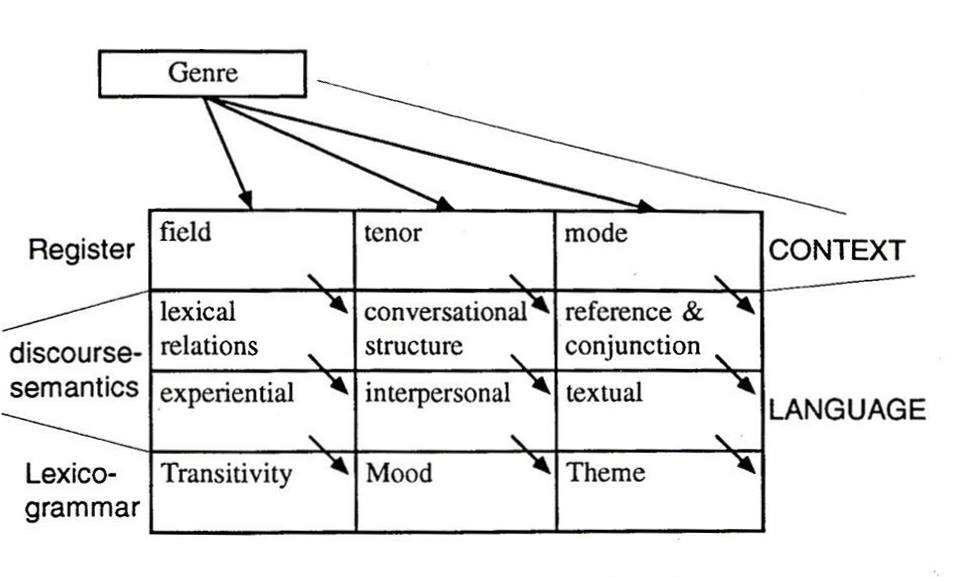
\includegraphics[width=0.65\textwidth]{../images/egginsfixed.jpg}}
\caption[Strata and metafunctions of language]{Strata and metafunctions of language (adapted from Eggins, 2004)}
\label{fig:eggins}
\end{figure}

\subsection{Affordances of \glsfmtshort{SFL} for researching an \glsfmtshort{OSG}}

\gls{SFL} has been applied to a diverse array of research areas including first and second language acquisition \cite{halliday1993towards,hasan_learning_1994}, language pedagogy \cite{halliday_towards_1993}, historical linguistics \cite{cummings2010introduction,martin_re/reading_2003} and (critical) discourse analysis \cite{hunston_systemic_2013,le_systematic_2009,martin_working_2003}. For the latter of these, \gls{SFL} is particularly useful, and has for this reason become one of the most popular grammars and theories of language for discursive research: as Halliday explains, at the most general level, \gls{SFL} is used `to understand the quality of texts: why a text means what it does, and why it is valued as it is' \parencite*[p.~xxx]{halliday_introduction:_2004}. In fact, from a systemic\hyp{}functional perspective, the use of a grammar is a prerequisite for all discourse analytic research. In Halliday's words,

\begin{quote}\small\singlespacing
it is sometimes assumed that discourse analysis, or `text linguistics' can be carried on without grammar---or even that it is somehow an alternative to grammar. But this is an illusion. A discourse analysis that is not based on grammar is not an analysis at all, but simply a running commentary on a text \parencite*[p.~xvii]{halliday_introduction:_2004}).
\end{quote}
%
%todo: reword again?
As a result of this conviction, the organisation and metalanguage of \gls{SFL} has in part been designed with text analysis in mind.

%todo: add zappavigna , hunston, cmc contexts...

The overall utility of \gls{SFL} for analysis of an \gls{OSG} may be divided into three main factors: the treatment of language as constitutive of text, the notion of language as a meaning\hyp{}making resource, and the division of interpersonal and experiential metafunctions within a grammar. These three factors are outlined below.

\subsubsection{Language as constitutive of context} \label{sect:context-in-text}

Though context is an increasingly central concern within many branches of linguistics, \gls{SFL} is notable for the extent to which its theory of context has been articulated and empirically applied \cite{widdowson_text_2008}. Halliday explains that in \gls{SFL}, context and text are in fact seen as `aspects of the same process', and that any sample of language use thus in fact `goes beyond what is said and written: it includes [...] the total environment in which a text unfolds' \parencite*[p.~5]{halliday_language_1989}. Therefore, \gls{SFL} treats language as constitutive of, rather than simply bound to, its context. As context can often be accurately deduced from text alone, and as context can be used to predict appropriate kinds of texts, some \gls{SFL} theorists contend that \emph{context is in text} \cite[e.g.][p.~7]{eggins_introduction_2004}. Context and language thus together construct both a reality and roles for people within it \cite{veel_learning_1997}.

This notion of language as simultaneously constructing and responding to the demands of contexts of situation has often formed an implicit theoretical assumption in online community and \gls{OSG} research: many works reviewed in the previous chapter tacitly take the perspective that language \emph{must} be responsible for the development of distinct cultures in online groups, as language is often the sole semiotic system available to group members \cite{thorne_computer-mediated_2008}.

%The absence of research explicitly drawing upon \gls{SFL} for online discourse socialisation research is thus striking.

\subsubsection{Language as a meaning-making resource}

The \glslink{SFL}{systemic\hyp{}functional} approach foremost involves an understanding of language as a semiotic system strategically drawn upon by language users as a meaning\hyp{}making resource---`how people use language with each other in accomplishing everyday social life' \cite[p.~2]{eggins_introduction_2004}. The orientation of the theory toward function and meaning\hyp{}making may be contrasted with phrase structure grammars, which typically do not attempt to account for meaning or pragmatics, and which are not grounded in analysis of realised linguistic patterns, but instead seek to provide rules that conform to speakers' intuitions regarding what is grammatically possible to say \cite{martin_english_1992}. \gls{SFL}, in contrast, understands language as \emph{purposive}: its use is motivated by purposes that may or may not be transparent or tangible. This is an appropriate theoretical stance for investigations of linguistic choices in an online community, because all communities are inherently social, and because in text\hyp{}based \gls{CMC} language is the main resource upon which members can draw to achieve their respective goals.

%\paragraph{Quantifiability of linguistic features}
%Halliday explains that it is possible to evaluate texts by counting the frequencies of relevant phenomena...
%Halliday remarks on the potential usefulness of very large datasets \parencite*{halliday_language_1992}
%This is amenable to the corpus-based approach taken here.

\subsubsection{Interpersonal and experiential functions of language}

%todo: add a ref to harvey so it doesn't seem like a fudge
From a systemic perspective, the simultaneous provision of health information and social support within \glspl{OSG} is realised by \glslink{member}{users} attending simultaneously to two metafunctions of language: an interpersonal dimension, responsible for negotiating role relationships, and an experiential dimension, responsible for communicating propositions about the world. This is the most useful affordance of \gls{SFL} for investigation of \glspl{OSG}, because the division of types of meaning is central to the reason for the community's existence: if the social element were not desired, \glslink{member}{users} would likely be content to simply read from static pages; if experiential content were not desired, health communities and the threads within them would not need to be organised by topic and subtopic. The interest in the phenomenon of \emph{advice} noted in Section \ref{sect:advice} would likewise stand to benefit from clearer delineation of the relationship between social roles and ideational content, each of which occupies a distinct, but overlapping space within acts of advising or directing others to act. Such a delineation would likely not be unwelcome. Early conceptualisations of the process of social support bear striking resemblance to the systemic model of interpersonal meaning: \textcite[p.~11]{shumaker1984toward} remind us, for instance, that social support is foremost `an exchange of resources between two individuals'.

\subsubsection{\glsfmtshort{SFL} and corpus linguistics}

In systemic\hyp{}functional terms, the \gls{corpus} is a large collection of instances of language use. These instances are typically organised by register, or by register dimensions. Automated counting of patterns in these instances is one possible way to uncover the grammar---that is, the patterns that generalise across the instances. A particular benefit of \gls{CL} approaches is that they make it possible to sketch out the probabilities of certain choices in certain contexts. At the same time, \gls{CL} approaches can test key tenets of \gls{SFL} theory \cite{honnibal_creating_2007}. \textcite{clarke_patterns_2012}, for example, uses a corpus-based approach to test the context metafunction hookup hypothesis---that is, the connection between language and context.

\gls{CL} and \gls{SFL} also share a number of underlying similarities. Most obviously, both are concerned with analysis of natural language, and both share a conceptualisation of \emph{register} as playing a significant role in shaping the \glslink{lexicogrammar}{lexicogrammatical} patterns to be found within texts \cite{hunston_systemic_2013}. Another key point of convergence between \gls{SFL} and \gls{CL} is in the treatment (explicit in \gls{SFL}, generally implicit in \gls{CL}) of context as being \emph{contained within} instantiated texts---`context is in text', rather than around it \cite{eggins_introduction_2004}. Systemicists evidence this assertion through the fact that we can often accurately deduce the overall functions, purposes and genres of highly decontextualised fragments of texts: \emph{Submissions must contain 8--10 references} can be quickly identified as part of a set of instructions for the submission of academic work, based purely on its lexical (submissions, references) and grammatical (nominalisation, modalisation, etc.) properties. In the same way, Halliday conceptualises \glslink{lexicogrammar}{lexicogrammatical} features of texts as probabilistically determined by their context. That is to say, a given constellation of interpersonal, experiential and textual variables (e.g. the writing of a professor to undergraduates in a written course overview) will likely contain the kinds of \glslink{lexicogrammar}{lexicogrammatical} features described in the example above \cite{halliday_corpus_1991}. This conceptualisation is of great benefit to corpus linguists interested in discourse analysis: given that \gls{CL} methods inherently involve the stripping of contextual information from natural language, and that analysis of contextualised language is preferred within the discourse analytic tradition, the recognition of context within \gls{lexicogrammar} allows \gls{CL} practitioners to address the common claim  \cite[e.g.][]{virtanen_discourse_2009} that \glslink{CL}{corpus} and discourse linguistic approaches, having very different orientations toward context, are difficult to reconcile.

\subsection{Overview of relevant elements of \glsfmtshort{SFG}}

%ntodo: sfl glossary weirdness
The core of \gls{SFL} is its grammar, known as the \glsxtrfull{SFG}, which is organised along the three axes discussed above. In this section, I describe the parts of the \gls{SFG} that are most relevant to the case study. The major references for this section include \citeauthor{halliday_introduction_2004} 2004, \citeauthor{matthiessen_lexicogrammatical_1995} 1995, and \citeauthor{eggins_introduction_2004} 2004.

\subsubsection{Register}

%todo: clean up, no repeating
Register occupies the level of abstraction above \glspl{discourse-semantic}, where language interfaces with a context of situation. The total content of each metafunction (interpersonal, experiential and textual) respectively corresponds to the three register variables of \emph{Tenor}, \emph{Field} and \emph{Mode} \cite{halliday_language_1989}. Halliday provides a minimal definition of each component:

\begin{enumerate}
\item  `The \sctext{Field of discourse} refers \emph{to what is happening}'
\item `The \sctext{Tenor of discourse} refers to \emph{who is taking part}'
\item `The \sctext{Mode of discourse} refers to \emph{what part the language is playing}' \parencite*[p.~12]{halliday_language_1989}
\end{enumerate}
%
In \gls{SFL}, doing register analysis can refer either to creating qualitative descriptions of the Field, Tenor and \gls{Mode} of a text (or collection of related texts), or to the process of generating quantitative, corpus\hyp{}based models of these features \cite{lukin2011halliday,matthiessen_modeling_2015}. Qualitative descriptions are intended to provide `[an interpretation of] the social context of a text, the environment in which meanings are being exchanged' \cite[p.~12]{halliday_language_1989}. Quantitatively, the internal dimensions of a single register can be modelled by counting relevant \glslink{lexicogrammar}{lexicogrammatical} features. The distribution of Process Types and the participants engaged in them, for instance, can be used to determine how speakers construe the world around them; \sctext{Mood} features can be analysed in order to see how speakers position themselves with respect to others (see below). 

Using a cartographic metaphor, \textcite{matthiessen_modeling_2015,Matthiessen2015} calls for further work within functional linguistics that models the internal dimensions of registers, and then situates these models within a cluster of related registers (presented later as Figure \ref{fig:pie-of-fortune}). By comparing these distributions to those found in other registers, registers can be arranged as a landscape, either along the axis of stratification or instantiation. The ultimate, perhaps distant goal, is to synthesise information about individual registers, in order to form a description of the meaning potential of a language, realising the notion of language as `an assembly or assemblage of registers' \parencite*[p.~44]{matthiessen_modeling_2015}. 

\textcite{matthiessen_applying_2013} has also applied register analysis to the domain of healthcare. Within the \gls{consumercentred} paradigm, this means focussing on individual healthcare consumers' health journeys, rather than on, for example, how consumers move through a given hospital or clinic in general. These healthcare journeys, Matthiessen explains, consist of sequence of encounters with formal and informal healthcare institutions. Each encounter presents a registerial configuration of topic, interactants and media: we may speak with a doctor in a busy clinic about our symptoms, or to a mental health practitioner about our personal relationships in an hour\hyp{}long consultation; we may phone an insurance carrier to clarify an issue about coverage, and write to a family member on Facebook about what we have learned. The case study of this thesis, centred on the registerial environment of an \gls{OSG}, has yet to be described within \gls{SFL} or \gls{HC} literature. The registerial description provided in Chapter \ref{chap:discuss-bp} is therefore intended to facilitate the addition of this register to the current body of knowledge and descriptions of the kinds of registers that may be encountered within consumers' journeys beyond the clinic.

%These meanings are realisations within the \sctext{Mood} and \sctext{Transitivity} choices that \gls{Forum} \glspl{member} make in their \glspl{post}. The two metafunctions and their implicated grammatical systems are described below. Chapters \ref{chap:researchdesign}--\ref{chap:experiential} combine to provide a quantitative model of the register of the \glslink{Forum}{Bipolar Forum}. Chapter \ref{chap:discuss-bp} presents a qualitative summary of Field, Tenor and Mode.

\subsubsection{Interpersonal meanings, MOOD and MODALITY} \label{sect:mood}

The Tenor variable of register is realised by interpersonal meanings. In turn, these meanings are made via the \sctext{Mood} and \sctext{Modality} systems of the \gls{lexicogrammar}. The interpersonal metafunction is responsible for negotiating role\hyp{}relationships with other speakers. It thus facilitates a constant \emph{exchange} of material and semiotic commodities; it is used to \emph{enact}, and to \emph{interact}.

\paragraph{Speech Function and Mood\slash Indicative Type}

In the \gls{SFG}, at the broadest level, utterances involve two potential \emph{speech roles}: \emph{giving} and \emph{demanding}. Within either speech role, two types of commodities may potentially be given or demanded: \emph{information}, or \emph{goods and services}. This leads to four main \emph{speech functions}, each of which is congruently realised by a different \sctext{Mood Type}. Information is given via statements, which are realised with declarative Mood. Information can be demanded via questions, congruently realised with the interrogative Mood. Goods and services are given via modalised declaratives. Demands for these non\hyp{}semiotic commodities are made via commands, which are realised with (non-indicative) imperative Mood. These intrastratal relationships are summarised in Table \ref{tab:roles}.

\begin{table}[htb]
\centering\small
\begin{tabular}{lll}

\toprule
\textbf{} & \textbf{Information} & \textbf{Goods and services} \\ 
\midrule
\textbf{Giving}   & statement $\rightarrow$ declarative    & offer $\rightarrow$ modalised interrogative     \\ 
\textbf{Demanding}   & question $\rightarrow$ interrogative & command $\rightarrow$ imperative    \\
\bottomrule
\end{tabular}
\caption[Mood Type and Speech Function]{Speech roles, commodities, speech functions and congruent \sctext{Mood Types} in SFL}
\label{tab:roles}
\end{table}   

\paragraph{Grammar of the \sctext{Mood} system} \label{sect:mood-grammar}

Each indicative clause contains a \emph{Mood Block}, comprised of a \emph{Subject} and \emph{Finite}. Optionally, clauses may also contain a \emph{Residue Block}, which can include a \emph{Predicator}, a \emph{Complement}, and\slash or one or more \emph{Adjuncts}. As non-indicatives, imperatives are comprised entirely of the Residue Block. In the case of declaratives, to determine which element is the Mood Block, a reverse-polarity tag can be added to the end of the declarative:

\begin{quote}
Geoff had difficulty with the task, \emph{didn't he?}
\end{quote}
%
Whatever is referenced by the pronoun in the tag is the Subject component of the Mood Block. The Finite is the first verb or modal in the verbal group that follows. It too is duplicated in a tag question in the case of \emph{be}, \emph{have} or a modal Finite; it is replaced by \emph{do} in other cases. The \emph{Polarity}, which is often unmarked when positive, is the opposite of the polarity in the tag. These elements together form the Mood Block. What remains in the clause is the Residue.

Residue also has component parts: the \emph{Predicator} is the part of the verbal group that carries a sense of the actual process undertaken. When a clause has only a single-word verbal group, it functions as both Finite and Predicator. If there is secondary tense information such as a progressive element, it is realised in the Predicator \cite{halliday_introduction_2004}. Residue may also contain a \emph{Complement}. The Complement is what becomes Subject if the clause is passivised. Finally, \emph{Adjuncts} are elements of the Residue that contribute non-essential information. Generally realised by adverbial or prepositional groups, Adjuncts cannot be turned into Subjects through passivisation.

Adjuncts may be \emph{circumstantial} (experiential), \emph{modal} (interpersonal), or \emph{textual} (thematic). Circumstantial adjuncts are those that add information concerning cause, time, matter or agent (discussed in the next section). Modal adjuncts\endnote{A fuller account of the differences and tests needed to differentiate mood adjuncts has been provided by \textcite{eggins_introduction_2004}.}~provide information concerning mood or polarity, or comment (the speaker's assessment of the clause) or vocative (naming speakers for addressal, turn\hyp{}taking, etc.). Finally, thematic adjuncts may have the role of facilitating conjunction or continuity with other clauses.

Importantly, some Mood Adjuncts are realised through \emph{grammatical metaphor}---that is, when what is congruently expressed through one rank or component is expressed through another.
%
\begin{multicols}{2}
\begin{quote}
\sctext{Grammatical metaphor}

\emph{I think} he came back.
\end{quote}

\begin{quote}
\sctext{Congruent form}

= \emph{Perhaps} he came back.
\end{quote}
\end{multicols}
%
\noindent \emph{I think}, for example, involves a grammatical metaphor---in this case, upward rank shift, where meaning typically realised by a word (in this case, a modal operator or Mood adjunct) is realised by an entire clause \cite{halliday_concept_1966,taverniers_systemic-functional_2002}. The fact that \emph{I think} is functioning as a constituent, rather than as an independent clause, can be ascertained by the tag question test: in the examples below, we can see that \emph{he} and \emph{'s} are typically the Subject and Finite within the Mood adjunct:

\begin{multicols}{2}
\begin{quote}
I think he's OK, \emph{isn't he?}
\end{quote}

\begin{quote}
*? I think he's OK, don't I?
\end{quote}
\end{multicols}
%
\noindent Because \emph{I think} is not functioning as an independent clause, it `play[s] no part in the structure of the interaction' \cite[p.~162]{halliday_introduction_2004}.

Differences in Indicative\slash Mood Type are realised by different configurations of the Subject, Finite and Predicator. For polar interrogatives, the Finite and Subject simply switch places. Aside from copula constructions, whenever the Finite and Predicator are realised with the same word, the operator \emph{do} must be inserted as the Finite for interrogatives:

\begin{multicols}{2}
\begin{quote}
\emph{Have you gone this week?}
\end{quote}
\begin{quote}
\emph{Do you know the way?}
\end{quote}
\end{multicols}
%
\noindent For WH\hyp{}Interrogatives, `the WH\hyp{}element is always conflated (mapped onto, fused with) another element of clause structure' \cite[p.~175]{eggins_introduction_2004}. It may potentially be mapped onto Subjects, Complements or circumstantial Adjuncts. Whichever element it is mapped onto is the same element needed in a minimally satisfactory reply:


\begin{multicols}{2}
\begin{quote}
\emph{Who moved the table?}

\emph{When did he do it?}
\end{quote}
\begin{quote}
\emph{Mahsa.}

\emph{An hour or two ago.}
\end{quote}
\end{multicols}

%
\noindent The Mood structure of basic imperatives involves removing the Mood element altogether:

\begin{multicols}{2}
\begin{quote}
\sctext{Interrogative\slash question}

\emph{Have you been taking} your meds?
\end{quote}

\begin{quote}
\sctext{Imperative\slash command}

\emph{Take} your meds.
\end{quote}
\end{multicols}

%\begin{multicols}{2}
%\begin{quote}
%\emph{Go to where the pepper grows!}
%\end{quote}
%\begin{quote}
%\emph{Let him speak!}
%\end{quote}
%\end{multicols}

% Imperatives involving \emph{let} are treated unusually by SFG \cite{huddleston_constituency_1988}. \emph{Let} is seen as `enabling the expression of the subject', and is thus treated within the subject component of the Mood Block:\endnote{Other varieties of English imperative such as \emph{`Don't you take my copy of the Bostonians'} are analysed in \textcite[pp.~184--5]{eggins_introduction_2004}}~

\paragraph{Metaphorical realisations of Speech Function}

The correspondence between interpersonal semantics and \sctext{Mood} choices is not always one\hyp{}to\hyp{}one. In situations where interactants are of a relatively equal social status, incongruence between Mood Type and Speech Function emerges as a politeness or hedging strategy. In particular, commands may be realised through alternative Mood Type choices (Table \ref{tab:gram_met_mood}). The most appropriate and\slash or likely choice is dependent on the overall Tenor of an interaction, and on who is speaking. In unequal relationships, the higher status participant tends toward congruent, imperative realisations of commands, while the lower status participant opts for incongruence (\emph{Would you be so kind as to ...}).

\begin{table}[htb]
    \begin{tabular}{ll}
    \toprule
    Mood type & Realisation \\
     \midrule
    Command & \emph{Go back on the meds.} \\
    Declarative & \emph{I think you should go back on the meds} \\
    Interrogative &  \emph{Why don't you go back on the meds?} \\
    Mod. declarative & \emph{I would go back on the meds (if I were you).} \\
    \bottomrule
    \end{tabular}
\caption{Grammatical metaphor as politeness strategy}
\label{tab:gram_met_mood}
\end{table}
%
As reviewed in the previous chapter, the relationship between congruence of \sctext{Mood Type} selection and the role relationships of speakers in an interaction has already been noted in the context of advice provision by \textcite[see Section \ref{sect:advice}]{decapua_`if_1995}. Accordingly, in an \gls{OSG}, we can expect that the role-relationship disparity between long and short term users may manifest linguistically in imperative commands being issued by veterans, with the proportion of advice issued via imperatives increasing with the membership length of the veteran member. Notably, this kind of incongruence poses a challenge for corpus\hyp{}based methods.

%\begin{enumerate}
%    \item Go back on the meds.
%    \item I think you should go back on the meds % this is modulated! :(
%    \item Why don't you go back on the meds?
%    \item I would go back on the meds (if I were you).
%\end{enumerate}

\paragraph{MODALITY} \label{sect:modality}

\sctext{Modality} is a key resource within the interpersonal exchange. It is realised within Mood structure in two ways: \emph{modalisation} and \emph{modulation} \cite[p.~179]{eggins_introduction_2004}. Functionally, modalisation is when a speaker makes meaning related to the \emph{probability} or the \emph{usuality} of an event: as Eggins explains, `modalisation is the expression of the speaker's attitude towards what s\slash he's saying' \parencite*[p.~180]{eggins_introduction_2004}. Grammatically, modalisation may be realised through Mood adjuncts (as explained earlier), a modal operator, or both at the same time. In every case, the modal elements are gradable. 

\setlength{\columnsep}{-5mm}
\begin{multicols}{3}\raggedright{
\begin{quote}
\sctext{Mood adjunct}

\singlespacing{She \emph{certainly} knew the text well.}
\end{quote}
\begin{quote}
\sctext{Modal operator}

\singlespacing{Power \emph{may} have been restored.}
\end{quote}
\begin{quote}
\sctext{Both together}

\singlespacing{I \emph{could sometimes} win.}
\end{quote}
}
\end{multicols}
%
% does this fit?
Modals may therefore be expected to appear in a number of situations within an \gls{OSG}, including marking of hesitation by newcomers \cite{vayreda_social_2009,weber_missed_2011}, and in veterans' polite sharing of information and potential actions.

\paragraph{POLARITY}

\sctext{Polarity} is the binary opposition between positive and negative. In \gls{SFL}, \sctext{Polarity} is primarily considered an interpersonal feature, since in contracted forms it becomes attached to the Finite \cite[p.~143]{halliday_introduction_2004}. It represents the two poles of certainty, with modalisation and modulation construing various levels of certainty and uncertainty in between. \textcite{halliday_introduction_2004} provide corpus evidence that clausal \sctext{polarity} is positive in 90 per cent of cases; negative polarity, they claim, is always the marked variant. Its meaning, however, is highly dependent on the content of the clauses to which it responds, functioning as affirmation or denial of the validity of the previous proposition or proposal. As such, it is difficult to track using existing corpus methods. This difficulty is exacerbated in the case study, which treats individual \glspl{post}, rather than \glspl{thread}, as the unit of analysis. Though the proportion of responses that affirm or deny the content of the previous clause would no doubt shed light on the extent to which exchanges are harmonious or contentious, this is unassessable without shifting the unit of analysis to the \gls{thread}, which would in turn make difficult the analysis of how language use changes over the course of membership. \sctext{Polarity} is therefore accounted for in the case study mostly for the sake of completeness of the overall analysis of the \sctext{Mood} system, and the interpersonal meanings the system is responsible for realising.

\subsubsection{Experiential meanings and the system of TRANSITIVITY} \label{sect:trans}

As explained earlier, clauses in \gls{SFL} are multifunctional units. At the same time as interpersonal relationships are enacted and negotiated through choices of \sctext{Mood} and \sctext{Modality}, experiential meanings are being expressed via the \sctext{Transitivity} system. Through this metafunction, speakers make \emph{representations} of inner and outer states, and of Things in the world and Events that they are involved in. In each clause, language users are \emph{construing} reality as change, which may affect or be affected by participants. Coherent clause complexes therefore represent sequences of change.

In \gls{SFL}, the \sctext{Transitivity} system can be analysed from two complementary perspectives: the \emph{transitive model}, in which processes are grouped according to types, and the \emph{ergative model}, where processes are bound to Mediums, through which they are made possible and therefore, without whom they cannot exist.

\paragraph{Transitive model}

In the transitive model, the clause is structured around a \emph{process}, indexed mostly by the Event---that is, the rightmost verb in the verbal group (and prepositions, for phrasal verbs):

\begin{multicols}{2}
\begin{quote}
\emph{i \textbf{consider} myself blessed having you guys}  % user-goody2shuz-863.txt.xml
\end{quote}
\begin{quote}
\emph{Oh \dots and her ex bf glen \textbf{broke up with} his gf} % user-goody2shuz-927.txt.xml
\end{quote}
\end{multicols}
%
\noindent This process must belong to a \emph{Process Type}. Process Types are distinguishable based foremost on lexis, but also on the grammar of the clause they head. Various syntactic and\slash or semantic tests can be used to disambiguate more difficult cases, though accurate Process Type identification by both human and machine has often proven challenging \cite{odonnell_survey_2009}. Each Process Type constrains the available configurations of participants (nominal groups) and circumstances (adverbial or prepositional phrases) in the clause. A summary of Process Types, identification tests and associated participant roles is given in Table \ref{tab:proctypeoverview}.

\begin{table}[htb]
\begin{tabularx}{\textwidth}{lXXXXX}

\toprule
\#~ & Process Type & Definition & Typical verbs & Identification test & Participants \\ \midrule
1.  & Material       & Doing tangible things         & \emph{kick, give, draw}   & \emph{What did x do?}        & Actor (goal) (range) (beneficiary) \\
2.  & Mental         & Thinking or feeling           & \emph{think, believe}    & \emph{What do you think, feel or know about y?}      & Senser, phenomenon        \\
3.  & Verbal         & Saying            & \emph{shout, yell, tell}    & \emph{What did x say?}       & Sayer, (receiver) (verbiage)   \\
4.  & Behavioural       & Psychological and \newline physiological behaviour & \emph{cough, smile, dream}  & Unmarked present tense has continuous sense            & Behaver (behaviour) (phenomenon)    \\
5.  & Existential       & `There' clauses            & \emph{be }      & Presence of non-locative \emph{there}    & Existent       \\
6a. & Relational \newline (ident.)   & Ways of being           & \emph{equal, mean, symbolise}  &  \emph{x is a member of the class a.}    & Attribute, carrier      \\
6b. & Relational \newline (attr.)   & Defining             & \emph{own}      & \emph{x serves to define the identity of y.}   & Cannot be passivised     \\
\bottomrule
\end{tabularx} 
\caption{Summary of Process Types}
\label{tab:proctypeoverview}
\end{table}

\FloatBarrier
\paragraph{Ergative model}

The ergative model of \sctext{Transitivity} conceptualises each clause as a quantum of change in the world, centred on a Process being carried out through a Medium. When the causer of the change is not mentioned, the result is a \emph{middle clause}---a construal of a \emph{happening}. In cases where the Medium does not bring about the process, an Agent may also be added (resulting in an \emph{effective clause}, or a \emph{doing}).

\begin{multicols}{2}
\begin{quote}
\small
\noindent \sctext{Medium + Process: Happening}

\noindent \emph{my dd is hitting manic mode and i think it 's time} 
\end{quote}

\begin{quote}
\small
\noindent \sctext{Agent + Process + Medium: Doing}

\noindent \emph{you hit a nerve and i felt the need to stand up for myself} % user-DB1973-9.txt.xml
\end{quote}
\end{multicols}
%
\noindent A critical difference between transitive and ergative models is that core participant roles can be disambiguated in the ergative model simply by checking for the existence of multiple nominal group arguments of a process: a two\hyp{}participant process will likely contain a \emph{Medium} and an \emph{Agent}, while a single\hyp{}participant process will be a Process\hyp{}Medium configuration. For corpus\slash computational linguistics, the ergative model therefore represents an ability to more easily identify agency, which can be expected to play an important role in the way participants in a Field of discourse are construed. That said, the transitive model is equally useful, highlighting experience of certain types of change by social actors. The two models are complementary; each is drawn upon in the analysis of \sctext{Transitivity} (Chapter \ref{chap:experiential}) according to its strengths.

%\begin{figure}[!ht]
%\centering
%\includegraphics[width=3in]{../../images/circ}
%\caption[System of circumstance]{System of circumstance (from Eggins, 2004)}
%\label{fig:circ}
%\end{figure}

%\paragraph{Theme: textual metafunction} \label{sect:theme}

%`The Theme is the element which serves as the point of departure for the message, it is that with which the clause is concerned' or again `the Theme is the starting-point for the message; it is what the clause is going to be about''. \cite[p.~158]{huddleston_constituency_1988}

%`In English, Halliday says, the Theme is identifiable as `that element which comes in initial position in the clause''' \cite[p.~158]{huddleston_constituency_1988}

% paragraph theme_textual_metafunction (end)



%todo: doesn't flow from previous
\subsubsection{Context of culture: genre and ideology} \label{sect:genre}

%todo: copy edit
While the case study of the thesis for the most part involves methods drawn from \gls{CL}, the analysis begins with a generic (i.e. genre\hyp{}based) interpretation of \glslink{post}{contributions} to the \gls{Forum}. For this reason, in this section, I provide a basic overview of a conceptualisation of genre that has emerged from the \glslink{SFL}{systemic-functional} school, and an associated method for performing genre analysis.\endnote{It is important to note that the interpretation of genre as a level of abstraction greater than that of register is a development rejected within the `Hallidayan' approach to SFL \cite{lukin2011halliday}. The genre analysis in Chapter \ref{chap:introdata} is performed because it elucidates in an intuitive way how Forum interactions may proceed in identifiable sequences, and how the probabilities for lexicogrammatical features are different within each sequence. Theoretical issues of language and context, such as where in the hierarchy of stratification the lexicogrammatical probabilities are set, and whether or not genre stages themselves reconfigure the probabilities, are not issues covered in this thesis.}

%there are \cite[e.g.][]{fawcett_theory_2000}

In contrast to the context of situation, which concerns the environment in which a given text is produced, the context of culture refers to the broader conditions common to texts. Culture is the highest level of abstraction in \gls{SFL}---all other meaning systems exist within and belong to cultures \cite{halliday_language_1989}. Thus, the context of culture is the semiotic potential of the totality of sign systems. 

The best\hyp{}articulated component of the context of culture is the notion of \emph{genre}---that is, `recurrent configuration[s] of meaning, phased in discourse as a staged, goal-oriented social process' \cite[p.~9]{martin_genre-based_2013}. Genres ultimately derive their meaning from their instantiation within a given culture \cite[p.~99]{halliday_language_1989}. Though genre and register alike are realised by the contextual variables of Field, Tenor and Mode, genre theory emphasises the social purpose of the activity being undertaken in the text \cite{christie_genre_2005,martin_english_1992}. Thus, genres may be characterised as constellations of Field, Tenor and Mode that are culturally recognised as performing social functions \cite{eggins_introduction_2004}. It is also important to bear in mind when considering genre that individual genres are not necessarily distinct: \emph{macro-genres} may contain \emph{micro-genres}: the macro-genre of the \emph{essay}, for instance may draw on micro-genres of \emph{expositions}, \emph{discussions} and \emph{evaluative accounts}.

\textcite{eggins_analysing_2004} provide simplified, actionable parameters for performing systemic\hyp{}functional genre analysis. The six steps are outlined below.

\paragraph{Recognising a generic text}

Given that genres are culturally recognised by their very nature, simple reading of texts by those fluent in the relevant culture may be enough to identify the existence of a genre. For analysts and interactants alike, genres are recognised when texts appear to `move through predictable stages' \parencite*[p.~213]{eggins_analysing_2004}. \textcite{eggins_introduction_2004} argues that the existence of a word for the kind of behaviour seen in the text (i.e. \emph{purchasing}, \emph{commentating}, \emph{gossiping}) may at the very least be a clue that a potentially definable genre exists.

\paragraph{Defining the social purpose of the generic text}

This step involves clarifying the overall function(s) of a genre with as much specificity as possible---rather than `telling a story', sub\hyp{}categorisations such as `anecdote' or `exemplum' are more useful, given the existence of micro- and macro\hyp{}genres. More theoretically, this task also involves developing an understanding of how the genre constructs a social reality: by virtue of their existence alone, recognisable genre stages may provide insight into social practices and culturally accepted attitudes and values. 

\paragraph{Identifying and differentiating stages within a genre}

After breaking down the text into clauses as with \glslink{lexicogrammar}{lexicogrammatical} analysis, groups of these clauses must be divided by their role within the text. These roles should be functionally, rather than formally defined: \emph{Abstract} or \emph{Resolution} is superior to \emph{Beginning} or \emph{Chapter Three} because the latter are not genre specific. By convention, each of these functions should then in turn be described in prose.

\paragraph{Specifying obligatory, optional and recursive stages}

Stages may be obligatory, optional or recursive. Obligatory elements are considered to be defining features, and in some cases may be unique to the genre under investigation. Optional stages, on the other hand, are likely to be present in other genres. \textcite{halliday_language_1989} remind us that optional stages do not occur randomly: in the \emph{buying and selling genre}, the number of customers in the store or the size of the line may affect whether or not a \emph{greeting} or \emph{sale initiation} takes place. Both optional and obligatory stages may be recursive, as in the case of the buying and selling genre, in which \emph{sale request}, \emph{sale enquiry}, \emph{sale compliance} and \emph{sale} may go through limitless iterations \cite[p.~61]{halliday_language_1989}.

\paragraph{Devising a structural formula}

The next task is to represent the genre structure. By convention, each genre stage is delineated by a caret (~$\hat{}$~). Optional stages are bracketed. Recursive stages are square-bracketed, with brackets followed by  \textsuperscript{n}.

A number of notion schemes for representing the relationship between genre stages have been proposed, and many have undergone revisions in order to be easier to render on a computer \cite{eggins_introduction_2004}. Problematic is that many \cite[e.g. those in][]{halliday_language_1989} are esoteric, and lagging behind the representational schemes of other grammars in terms of readability (Hovy, 1996). In fact, the development and use of unique means of expressing optionality and recursion is perhaps superfluous and ultimately unhelpful, given that comparatively well\hyp{}known systems such as \emph{regular expressions} could potentially represent generic structure in a format familiar to at least some non\hyp{}\gls{SFL} practitioners. 

A particularly important addition to structural representation of genre is Hasan's \parencite*{hasan_structure_1985} notion of \emph{generic structure potential}: that is, a maximally expanded representation of genre staging that exhausts all possibilities for additional optional stages and recursion.\endnote{It is important to distinguish generic structure potential from \emph{genre potential}---that is, `all the linguistically-achieved activity types recognised as meaningful (i.e. appropriate) in a given culture' \cite[p.~35]{eggins_introduction_2004}. In practice, this translates to every possible configuration of Field, Tenor and Mode.}

\paragraph{Analysing the semantic and \glslink{lexicogrammar}{lexicogrammatical} features for each stage of a genre}

As Hasan explains,

\begin{quote}\singlespacing\small
a text has many modes of existence and so it can be analysed at many different levels, with each contributing to our understanding of the phenomena involved \parencite*[p.~116]{halliday_language_1989}.
\end{quote}
%
\noindent Thus, relevant parts of \gls{SFG} may be operationalised in order to investigate the phenomena of interest: a researcher interested in power dynamics within a text, for example, would likely perform an analysis of features of the \sctext{Mood} system, as these are responsible for the management of role\hyp{}relationships between interactants. Simultaneously, this analysis provides a justification of the treatment of the text as instantiating a genre and of the clause complexes as instantiating generic stages. \textcite{eggins_analysing_2004} note that since \gls{lexicogrammar} can provide hints as to genre staging, this step of the analysis may render it necessary to reconsider the previous delineation of stages.

Genre may influence the \gls{lexicogrammar} of texts in two ways. First, as genres are configurations of register variables, texts within genres must necessarily conform at the level of lexicogrammar. In this way, a genre such as \emph{sports commentary} is likely to bring about language which experientially positions players, teams, umpires and coaches as the main participants. Second, different genre \emph{stages} may influence \glslink{lexicogrammar}{lexicogrammatical} decisions. The \emph{evaluation} stage within the \emph{storytelling} macro\hyp{}genre, for example, is likely to opt for a declarative Mood, while experientially, it can be assumed that mental and relational Process Types may occur.

\paragraph{Ideology in SFL}

Ideology has a complex history within \gls{SFL}, originally conceptualised as the most abstract analysable stratum of text\slash context, as the overarching determinant of the context of culture \cite{eggins_introduction_2004}. Later work, however, often refrains from accounting for ideology \cite[e.g.][]{matthiessen_key_2010}, or disavows its existence as a distinct stratum within the hierarchy of stratification \cite[e.g.]{martin_genre_2006}. Regardless of its exact status within \gls{SFL}, ideology is commonly discussed in the contexts of both \glspl{OSG} and socialisation, and, accordingly, is in need of a brief description here.

One way of conceptualising ideology is `from above'. As \textcite{banks2009ideology} explains, two texts with very similar Field, Tenor and Mode can nonetheless mean very different things: politicians with opposing views, for instance, may give speeches within more or less identical registers, while ultimately expressing different sets of values. Ideology can also be conceptualised `from below': ideological values may be found within lexicogrammatical and semantic patterns that are common within a text, but that are rarely subject to negotiation, controversy or debate by the interactants. Experientially, while `Field of discourse' refers to what is being directly spoken about in a text, ideology refers more to the taken\hyp{}for\hyp{}granted assumptions about these things and events. For example, while there is a great deal of argument about the efficacy of some kinds of alternative medicine in many \glspl{OSG}, there is generally much less debate about the value of treatment itself: treatment can lead toward health, and is almost always worth undertaking. Some ideological values in these communities, therefore, may be that \emph{that illness requires treatment}, because \emph{treatment can make you healthy again}. The controversy surrounding pro\hyp{}anorexia \glspl{OSG} \cite[see e.g.][]{chancellor_recovery_2016} stems from the fact that these communities advocate challenging widely held ideological values about health, weight, illness and treatment.

In this thesis, without taking a particular stance on the role of ideology within \gls{SFL}, the term can still be operationalised in the case study as a way of referring to the more or less unargued or inarguable components of discourse within the \gls{Forum}. It is important to bear in mind, therefore, that ideology may or may not be substantively different from \glspl{discourse-semantic} or register; rather, here, it is simply a way of thinking about what the language users in texts take for granted or consider common\hyp{}sense.

\subsection{Criticism of \glsfmtshort{SFL}}

Both the overall orientation of \gls{SFL} and its grammar have received a number of criticisms that deserve to be addressed. \textcite{van_dijk_text_2004}, for example, has taken issue with three main dimensions of \gls{SFL} as a linguistic theory in general. First and most broadly, he notes that its sheer density creates difficulty when a researcher seeks to use only relevant sections of the theory:  `not only are the terms (Field, Tenor, Mode) hardly transparent, as to their intended meanings, but also the usual---informal---descriptions of their meanings are barely enlightening' \parencite*[p.~341]{van_dijk_text_2004}. Second, he characterises \gls{SFL} as lacking sufficient engagement with potentially useful interdisciplinary perspectives: `there is very little inspiration from the many other approaches to context in linguistics and especially in anthropology, sociology or social psychology, at least in the analysis of the context' \parencite*[p.~342]{van_dijk_text_2004}. Finally, he points out that \gls{SFL} has avoided engaging with cognitive accounts of language, and therefore can have little to say about the reality of the meaning\hyp{}making process for speakers themselves.

%todo: copy edit
Indeed, each of the three points is in some sense valid. \gls{SFL} is terminologically dense---a necessary evil, according to Halliday's preface to his \emph{Introduction to Functional Grammar}, when formulating a theoretical account of something as complex as a human language.  Van Dijk's second point, regarding a lack of dialogue between \gls{SFL} is also accurate. At a terminological level, for example, key terms in \gls{SFL} such as \emph{Tenor} have been coined in order to avoid ambiguity---a more natural term might be \emph{tone}, but this term also has a phonological meaning. The claim that \gls{SFL} engages little with related traditions at both the level of terminological and beyond is not a baseless one, however: as a second example, the $650+$ page \emph{Introduction to Functional Grammar} does not once mention \emph{pragmatics}, though what is meant by pragmatics in related areas overlaps to a very significant extent with the systemic conceptualisation of interpersonal \glspl{discourse-semantic}.\endnote{Halliday has addressed a perceived lack of engagement with the field of pragmatics: Pragmatics, he argues `has always been simply the instantial end of the semantics. We don't need a separate discipline' \cite[p.~138]{thompson2001interview}.}

The third criticism, related to the lack of cognitive accounts, is the only one which has some bearing on the overall explanatory power of the theory. Here, Van Dijk is not alone in his criticism: \textcite{rohdenburg_cognitive_1996} has argued that the systemic account of preposition\slash object ordering in clauses with phrasal verbs (\emph{She put the fire out} vs. \emph{She put out the fire}) as being motivated by textual thematic demands (i.e. information structure, or givenness\slash newness) is only a partial account of the underlying motivations for speaker choices. Cognitive demands on addressees play an important role in choices between grammatical alternatives, with the likelihood of clause\hyp{}final preposition decreasing steadily as weight and length of the object grows \cite[c.f.][]{hawkins1992syntactic}. While a lack of engagement with cognition may have benefits for certain kinds of text analysis, as well as some computational tasks \cite{odonnell_[sys-func]_2014}, it is prudent to bear in mind that even if the systemic account may not in and of itself be incorrect, there is compelling evidence for its instead being in some respects only a partial account of how language works.

Others also critiqued the \gls{SFG}'s textual metafunction: \textcite{huddleston_constituency_1988} and \textcite{widdowson_text_2008} have problematised the notion of the \gls{Theme} as simply the first element in a clause, in cases where there are dummy subjects, for example. More generally speaking, Van Dijk has also further criticised what he sees as an attempt to force \glslink{lexicogrammar}{lexicogrammatical} \emph{conjunction} to line up with the register variable of \emph{Mode}. Perhaps this criticism is tacitly embraced by \textcite{eggins_analysing_2004}, who tend to advocate the use of terminology and concepts from \gls{CA}, rather than \gls{SFL}, for investigations of turn\hyp{}taking, overlap and the like. For these reasons, compounded simply by issues of scope, I have opted not to consider textual meanings in this thesis in any serious detail. This is perhaps unfortunate, as much could foreseeably be learned about \glspl{OSG} through analysis of the ways in which the take\hyp{}up of advice (for example) is realised in \gls{forum} \glspl{thread} (see Section \ref{sect:discuss-register} for a brief demonstration of the possible value of analysis of choices of Theme).

%Finally, it is worth noting that schisms exist within the overarching theory of \gls{SFL}, with the various factions tending to criticise



%\noindent In the context of \glspl{OSG}, the distinction between experiential, interpersonal and textual meanings allows the researcher to focus on components of the \gls{lexicogrammar} that realise the two major purposes of the community: health information provision can be investigated through experiential meanings and the Transitivity system, and social support and member role negotiation can be analysed by looking at how different Mood types (e.g. imperatives, declaratives, interrogatives) as well as Modality (communicating information regarding obligation, probability, usuality, etc). Accordingly, from a systemic functional perspective, we can predict that certain features of both Mood and Transitivity will be subject to change over the duration of membership. In terms of Mood and Modality, long term members would be more likely to provide information or suggest a course of action (congruently realised through declaratives and imperatives), while new members would request information (through interrogatives), and be very unlikely to issue commands. Furthermore, modalisation could be a resource for hedging claims to knowledge in newer members' posts, while veteran users may use modalisation to stress the obligations of less-knowledgeable members or the certainty of their own claims. In terms of experiential meanings, greater familiarity with community norms is likely to be observable through the instantiation of more elaborate taxonomies and configurations of participants and processes \cite{martin_english_1992}, with more nuanced distinctions being drawn over membership duration between more symptoms, medications, kinds of health professional, and so forth.%. Finally, the appraisal dimension of \gls{SFL} \cite[see][]{martin_language_2005} may also be subject to change throughout membership, as normative judgments of key participants and processes may evolve.

%In addition to face-to-face encounters, examples of anonymous self-dis- closure abound in today’s increasingly technological society. Crisis center hotlines provide the highly stressed caller with immediate feedback, which may simply involve listening, or may entail providing caring responses and referral services. Similarly, a growing number of radio talk shows provide participants with direct responses to their problems and listeners with vicarious information. The accelerated growth of home computers has provided an additional avenue for anonymous support. With the purchase of a modem, people can communicate with other “users”; programs have been developed to assist people in linking up with the resources of strangers (Van Gelder, 1983) \cite[p.~18]{shumaker1984toward}

%In \gls{SFL} and its expansions \cite[e.g.][]{martin_language_1984,christie_genre_2005}, culturally recognised constellations of these three variables are treated as \emph{genres}, within which other micro-genres may also be contained. In our case, the vast majority of texts under consideration are within the genre of newspaper article, with micro-genres such as sports-journalism, editorials, opinion articles and so on being differentiated by the appearance of different \glslink{lexicogrammar}{lexicogrammatical} choices within both mood (i.e. use of interrogative mood, modalisation to connote subjectivity/objectivity) and transitivity systems (what is being spoken about). 



%\subsection{\gls{SFL} and healthcare}

%\gls{SFL} practitioners have recently turned their attention to healthcare contexts. \textcite{matthiessen_applying_2013} demonstrates the potential use within the emerging paradigm of relationship centred healthcare, showing how we can map the patient journey through healthcare institutions.

%~\ \todo[inline,color=green!40]{\noindent More here on \gls{SFL} healthcare.}

%another one here that robyn uses

%\subsection{Relevant applications of \glsfmtshort{SFL}}

%\gls{SFL} has been applied for a broad range of purposes. Here, I focus on discourse analytic, \gls{CL} and computational applications.

%\todo[inline,color=green!40]{Redo this part!}

%\subsubsection{\glsfmtshort{SFL} and discourse analysis}

%The fact that \gls{SFL} provides a well-articulated means of connecting \gls{lexicogrammar} to meaning, discourse and register has made it a popular choice in (critical) discourse analysis.

%\todo[inline,color=green!40]{Summary here}


%\subsubsection{Computational \gls{SFL}}

%There have been many computational \gls{SFL} projects, focussing both on natural language generation and parsing. Focussing on parsing, early efforts encountered mixed results, with \cite{odonnell_uam_2005,odonnell_\gls{sfl}_2005} Some important work from this era remains copyright protected. For others, source-code has not been publicly released. More recently, Costetschi's approach has been to convert Stanford CoreNLP collapsed dependency annotations to a simplified systemic\hyp{}functional annotation through a rule-based system. Other work has centred on providing a web-based interface for manual tagging, from which automatic annotation can be learned (The Halliday Centre Tagger---see Wu, 2015).

% DANIEL with CCG

%Direct access to systemic features would indeed be preferable to the approach taken in this thesis, which is ad-hoc, wordlist based conversion of CoreNLP dependency annotation. A full treatment of issues with the approach is provided in Chapter 7.

% semantic parsing


%\subsection{Theoretical orientation}
%
%\gls{SFL} may be characterised as empirically driven and bound, probablistic, predictive and descriptive. A key notion in %\gls{SFL} is that functional definitions and distinctions extend as far as \glslink{lexicogrammar}{lexicogrammatical} distinctions can be reliably %made: distinctions between the different kinds of processes are evidenced by grammatical, rather than thematic %information. Alternative systems of Process Types (e.g. the Cardiff SFG) are intended more as a means of simplifying %the (at times very dense) distinctions made in the Sydney grammar.
%
%Contrastive distinctions between grammatical and ungrammatical constructions are thus of primary importance. %Probabalistic evidence (concerning words that are likely to collocate, or a trend toward passivisation of a certain %process, for example) is secondary. Probablistic parts of lexical or grammatical behaviour are inherently associated %with contrastive distinctions, but to widely varying extents. 
%
%Passivisation in signage, computer errors, etc. (\emph{Smoking is not allowed, Permission denied,} etc), is %predictable due to the fact that it is of little importance, or indeterminable, who would\slash could be the actor (%that is, the authority enforcing the rule) in the active version of the clause. Here, the phenomenon is closely tied %to the function of the message. On the other hand, though British and Raj collocate, and though in part this is due %to the close relationship between adjectival modifiers and nouns, the strength of the collocation is more to do with %historical circumstances: there have not been other kinds of Raj.
%
%Finally, it is worth noting that judgements based on native-speaker intuition alone are not meaningful for the %purposes of analysis, but are of course viable means of locating phenomena \emph{for} analysis.
%
%\gls{SFL} shares an unusual relationship with the prescriptive\slash descriptive debate. It is a profoundly functional %theory, but does indeed mark ungrammaticality in formal terms. This is a consequence of the goal of \gls{SFL} to provide a %description of grammatical systems. Ungrammatical utterances provide useful heuristics for L1 and L2 development, or %the particular functional aims of a speaker in a given interaction.
%
%\section{Interaffordances of the research areas}
%
%The combination of CMC, \gls{CL}s and \gls{SFL} presented here create some affordances. Some have been described %in existing literature; some are outlined for the first time here.
%
%\subsection{CMC and \gls{SFL}}
%
%\gls{SFL} has rarely been combined with studies of CMC.

% MACNAMARA 2010 cited as describing these IFG 2014 p. 42

%coffin?

%Focussing on a particular online support group stabilises certain systemic features. Most importantly, the contextual dimension of mode can be sketched fairly quickly, because users must use \emph{posts} to communicate. Though the site links to related communities (including, later in the evolution of the community, a dedicated space for friends and family of those living with bipolar disorder), these have an identical architecture. No other community-sanctioned spaces for further discussion appear to be provided.

%In the case of the bipolar forum, the most macro fields of discourse (bipolar disorder, mental health) are prescribed in the title and rules of the community. Off-topic information can be moved or deleted by administators at their discretion.


%\input{chapters/medical-nlp}

%todo: should this and the line below say 'literature review'?
\section[Chapter summary]{Summary: theories and methods for investigating online healthcare discourse}

The synthesis of literature presented in this and the previous chapter has involved four research domains:

\begin{enumerate}
	\item Computer mediated communication (CMC) as a Medium, and \glspl{forum} as a \gls{Mode}
	\item Healthcare communication (HC) as a Field
	\item Corpus linguistics (CL) as an approach for analysing digital linguistic data
	\item Systemic functional linguistics (SFL) as a framework for understanding language
\end{enumerate}
%
The argument made throughout the literature review is that by combining these areas, we can learn new things about online intra\hyp{}\gls{consumer} health discourse, as well as uncover new ways to learn things. Key claims from qualitative literature can be tested quantitatively with largely automatic \gls{CL} methods, and evidenced by translating observed discourses into their lexicogrammatical realisations. 

The next part of the thesis, which introduces the case study of a \gls{bipolar} \gls{OSG}, demonstrates the potentiality of combining \gls{CL} methods and \gls{SFL} theory for the analysis of \gls{CMC}. The systemic grammar and sophisticated corpus methods make possible nuanced kinds of corpus interrogation that differentiate interpersonal from experiential meaning\hyp{}making.

%In doing this, the divide between qualitative approaches to \gls{CMD} and quantitative approaches to improved healthcare through data mining can be bridged. Discourse can be brought into the purview of statistical approaches that have tended to focus on analysis of metadata; discourse\hyp{}oriented research can have more useful implications for real-world healthcare issues.


%\section{Chapter summary}

%In this chapter, I presented \gls{CL} as a possible approach to analysis of online health discourse, and \gls{SFL} as a means of understanding texts. From the synthesis of literature emerged the beginnings of a framework for repeatable, quantitative analysis of health discourse. In the next chapter, I operationalise the nascent framework through a case study of linguistic change in an \gls{OSG}.

%\bibliography{../references/libwin.bib}
